\chapter{Anillos}
\label{cap:anillos}

\ifdefined\separatechapter\bookbanner\fi

En este capitulo primero vamos a revisar rápidamente los números complejos y
luego introduciremos las nociones abstractas de anillo y cuerpo y veremos los
primeros ejemplos y propiedades básicas.

% % % % % % % % % % % % % % % % % % % % % % % % % % % % % %

\section{Números complejos}

En el capítulo anterior hemos recordado la construcción de los números
racionales $\QQ$ a partir de los números enteros $\ZZ$ y también la construcción
de los números reales $\RR$ a partir de $\QQ$. Ahora vamos a revisar la
construcción de los números complejos $\CC$ a partir de $\RR$. Se supone que
este material es familiar al lector, así que voy a omitir algunos detalles.

\vspace{1em}

Los \term{números complejos} pueden ser identificados con las
\term{expresiones formales}
$$z = x + yi,$$
donde $x,y\in \RR$. Las palabras ``expresión formal'' significan que
$$x_1 + y_1 i = x_2 + y_2 i \text{ si y solamente si }x_1 = x_2\text{ e }y_1 = y_2.$$

El número $x$ se llama la \term{parte real} e $y$ se llama la
\term{parte imaginaria} de $z$. Se usa la notación
$$\Re z \dfn x, \quad \Im z \dfn y.$$
El conjunto de los números complejos se denota por $\CC$.
El \term{plano complejo} es la identificación entre $\CC$ y $\RR^2$ dada por
$z \leftrightarrow (\Re z, \Im z)$.

\begin{figure}[h]
  \begin{center}
    \begin{tikzpicture}[x=2cm,y=2cm]

      \draw (60:1) node[circle,fill,inner sep=1.5pt, label=above right:{$z = x + yi$}] {};

      \draw[dashed] ({cos(60)},0) -- (60:1);
      \draw[dashed] (0,{sin(60)}) -- (60:1);

      \draw ({cos(60)},0) node[label=below:{$x$}] {};
      \draw (0,{sin(60)}) node[label=left:{$y$}] {};

      \draw[->] (-1,0) -- (+1.5,0) node[right] {$\Re$};
      \draw[->] (0,-1) -- (0,+1.5) node[above] {$\Im$};
    \end{tikzpicture}
  \end{center}
  \caption{El plano complejo}
\end{figure}

Las sumas están definidas \term{término por término}; es decir,
$$(x_1 + y_1 i) + (x_2 + y_2 i) \dfn (x_1+x_2) + (y_1+y_2)\,i,$$
y los productos se definen mediante la multiplicación de los números reales,
la identidad
$$i^2 = -1$$
y la \term{distibutividad}; es decir,
$$(x_1 + y_1 i) \cdot (x_2 + y_2 i) \dfn (x_1 x_2 - y_1 y_2) + (x_1 y_2 + x_2 y_1)\,i.$$

Notamos que para qualesquiera $x_1,x_2 \in \RR$ se tiene
\begin{align*}
  (x_1 + 0\cdot i) + (x_2 + 0\cdot i) & = (x_1 + x_2) + 0\cdot i,\\
  (x_1 + 0\cdot i)\cdot (x_2 + 0\cdot i) & = x_1 x_2 + 0\cdot i,
\end{align*}
y en este sentido la multiplicación compleja es una generalización
de la multiplicación de números reales. Los números reales se identifican con
el subconjunto formado por los números de la forma $x + 0\cdot i$, que también
se denotan por $x$.

\begin{observacionejerc}
  \label{obs:los-complejos-forman-un-anillo}
  Las sumas y productos cumplen las siguientes propiedades.

  \begin{enumerate}
  \item[1)]
    \begin{itemize}
    \item[a)] $(z_1+z_2) + z_3 = z_1 + (z_2+z_3)$ para cualesquiera
      $z_1,z_2,z_3 \in \CC$.

    \item[b)] El número $0 \dfn 0 + i\cdot 0$ cumple
      $$z + 0 = 0 + z = z$$
      para todo $z\in \CC$.

    \item[c)] $z + (-z) = (-z) + z = 0$ para todo $z = x+iy \in \CC$, donde
      $-z \dfn -x - iy$.

    \item[d)] $z+w = w+z$ para cualesquiera $z,w\in \CC$.
    \end{itemize}

  \item[2)] El producto es distributivo respecto a la suma:
    $$z\,(w_1 + w_1) = z w_1 + z w_2, \quad (z_1 + z_2)\,w = z_1 w + z_2 w$$
    para cualesquiera $z,w_1,w_2 \in \CC$.

  \item[3)] El producto es asociativo:
    $$(z_1 z_2) z_3 = z_1 (z_2 z_3)$$
    para cualesquiera $z_1,z_2,z_3 \in \CC$.

  \item[4)] El número $1 \dfn 1 + i\cdot 0$ cumple
    $$z\cdot 1 = 1\cdot z = z$$
    para todo $z\in \CC$.

  \item[5)] El producto es conmutativo:
    $$zw = wz$$
    para cualesquiera $z,w\in \CC$. \qedhere
  \end{enumerate}
\end{observacionejerc}

Para un número complejo $z = x + iy$ su \term{conjugado} se define mediante
$$\overline{z} \dfn x - iy.$$

\begin{observacionejerc}
  La conjugación cumple las siguientes propiedades:

  \begin{enumerate}
  \item[1)] $\overline{z+w} = \overline{z} + \overline{w}$ y
    $\overline{zw} = \overline{z}\cdot\overline{w}$ para cualesquiera
    $z,w \in \CC$.

  \item[2)] $\overline{\overline{z}} = z$ para todo $z \in \CC$.

  \item[3)] $\overline{z} = z$ si y solo si $z \in \RR$. \qedhere
  \end{enumerate}
\end{observacionejerc}

\begin{definicion}
  El \term{valor absoluto} de $z = x + yi \in \CC$ es el número real
  $$|z| \dfn \sqrt{z \overline{z}} = \sqrt{x^2 + y^2}.$$
\end{definicion}

Notamos que $|z| \ge 0$ y $|\overline{z}| = |z|$.

\begin{observacionejerc}
  El valor absoluto satisface las propiedades habituales:
  \begin{enumerate}
  \item[1)] $|z| = 0$ si y solamente si $z = 0$;

  \item[2)] $|zw| = |z|\cdot |w|$ para cualesquiera $z,w\in \CC$;

  \item[3)] se cumple la \term{desigualdad triangular}
    $$\Bigl| |z| - |w| \Bigr|\le |z+w| \le |z| + |w|$$
    para cualesquiera $z,w\in \CC$. \qedhere
  \end{enumerate}
\end{observacionejerc}

\begin{figure}[h]
  \begin{center}
    \begin{tikzpicture}[x=3cm,y=3cm]
      \draw (75:0.75) node[circle,fill,inner sep=1.5pt, label=above:{$z$}] (z) {};
      \draw (30:1.25) node[circle,fill,inner sep=1.5pt, label=right:{$w$}] (w) {};

      \draw (0,0) -- (z);
      \draw (0,0) -- (w);
      \draw (0,0) -- ($(z)+(w)$) node[circle,fill,inner sep=1.5pt, label=above right:{$z+w$}] {};
      \draw (z)[dashed] -- ($(z)+(w)$);
      \draw (w)[dashed] -- ($(z)+(w)$);

      \draw (0,0) node[circle,fill,inner sep=1.5pt, label=below left:{$0$}] {};

      \draw[->] (-0.25,0) -- (+1.5,0) node[right] {$\Re$};
      \draw[->] (0,-0.25) -- (0,+1.5) node[above] {$\Im$};
    \end{tikzpicture}
  \end{center}

  \caption{La desigualdad triangular}
\end{figure}

\begin{observacion}
  Para todo número complejo $z = x+yi \ne 0$ existe un número único
  $z^{-1} \in \CC$ tal que
  $$z z^{-1} = z^{-1} z = 1.$$

  \begin{proof}
    Dado que $z\,\overline{z} = |z|^2$, se ve que hay que tomar
    $$z^{-1} = \frac{1}{|z|^2}\,\overline{z} = \frac{x}{x^2+y^2} - \frac{y}{x^2+y^2}\,i.$$

    Este número es único porque si hay dos $w_1, w_2 \in \CC$ tales que
    $z w_1 = z w_2 = 1$, entonces
    \[ w_1 = w_1\cdot 1 = w_1\,(z w_2) = (w_1 z)\, w_2 = 1\cdot w_2 = w_2. \qedhere \]
  \end{proof}
\end{observacion}

\begin{observacion}
  Para cualesquiera $z,w \in \CC$, si se cumple $zw = 0$, entonces $z = 0$ o
  $w = 0$.

  \begin{proof}
    Si $zw = 0$, entonces, tomando los valores absolutos, se obtiene
    $|z|\cdot |w| = 0$, así que $|z| = 0$ (es decir, $z = 0$) o $|w| = 0$
    (es decir, $w = 0$).

    Otra prueba, usando los inversos: si tenemos $zw = 0$ y $z \ne 0$, entonces
    \[ w = 1\cdot w = z^{-1}z w = z^{-1} 0 = 0. \qedhere \]
  \end{proof}
\end{observacion}

Usando las \term{coordenadas polares} en $\RR^2$, podemos expresar cada número
complejo como
$$z = r\,(\cos\phi + i\sen\phi), \quad \text{donde }r = |z|, ~ 0 \le \phi < 2\pi.$$
Si $z\ne 0$, entonces los números $r$ y $\phi$ están definidos de modo único.
La expresión de arriba se llama la \term{forma trigonométrica} (o \term{polar})
de $z$.

\begin{figure}[h]
  \begin{center}
    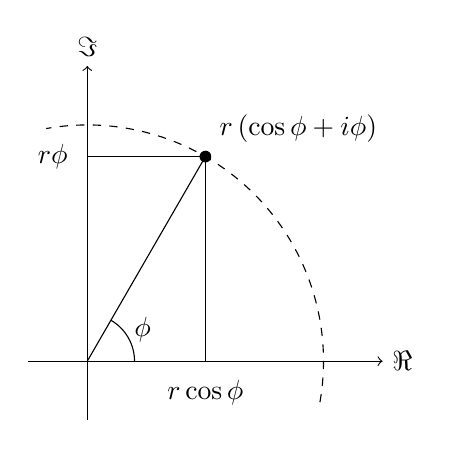
\begin{tikzpicture}[x=3cm,y=3cm]
      \draw[dashed] ([shift=(-10:1)]0,0) arc (-10:100:1);

      \draw (60:1) node[circle,fill,inner sep=1.5pt, label=above right:{$r\,(\cos \phi + i\sen\phi)$}] {};

      \draw ({cos(60)},0) node[label=below:{$r\cos\phi$}] {} -- (60:1);

      \draw (0,{sin(60)}) node[label=left:{$r\sen\phi$}] {} -- (60:1);
      \draw (0,0) -- (60:1);

      \draw (30:0.27) node {$\phi$};

      \draw (0.2,0) arc (0:60:0.2);

      \draw[->] (-0.25,0) -- (+1.25,0) node[right] {$\Re$};
      \draw[->] (0,-0.25) -- (0,+1.25) node[above] {$\Im$};
    \end{tikzpicture}
  \end{center}

  \caption{La fórma trigonométrica de números complejos}
\end{figure}

\begin{proposicion}[La identidad de Euler\footnote{\personality{Leonhard Euler}
    (1707--1783) --- matemático suizo, uno de los más prolíficos e importantes
    de toda la historia.}]
  Para cualquier $\phi$ se tiene
  $$\cos\phi + i\sen\phi = e^{i\phi}.$$

  \begin{proof}
    El coseno, seno y la exponencial pueden ser definidos mediante las series de
    potencias
    \begin{align*}
      \cos z & = \sum_{n\ge 0} (-1)^n\,\frac{z^{2n}}{(2n)!} = 1 - \frac{z^2}{2} + \frac{z^4}{24} - \frac{z^6}{720} + \cdots,\\
      \sen z & = \sum_{n\ge 0} (-1)^n\,\frac{z^{2n+1}}{(2n+1)!} = z - \frac{z^3}{6} + \frac{z^5}{120} - \cdots,\\
      e^z & = \sum_{n\ge 0} \frac{z^n}{n!} = 1 + z + \frac{z^2}{2} + \frac{z^3}{6} + \frac{z^4}{24} + \frac{z^5}{120} + \frac{z^6}{720} + \cdots
    \end{align*}
    ---es fácil recordarlas: basta memorizar la serie de $e^z$, y luego $\cos z$
    y $\sen z$ tienen series parecidas, pero alternantes; siendo una función
    par, $\cos z$ consiste en términos pares, y siendo una función impar,
    $\sen z$ consiste en términos pares. Calculamos que las potencias de $i$ son
    $$i^{2n} = (-1)^n, \quad i^{2n+1} = (-1)^n\,i.$$
    Luego,
    \[ e^{i\phi} =
      \sum_{n\ge 0} \frac{(i\phi)^n}{n!} =
      \sum_{n\ge 0} \frac{i^n\,\phi^n}{n!} =
      \sum_{n\ge 0} (-1)^n\,\frac{\phi^{2n}}{(2n)!} + i\,\sum_{n\ge 0} (-1)^n\,\frac{\phi^{2n+1}}{(2n+1)!} =
      \cos \phi + i\sen \phi. \qedhere \]
  \end{proof}
\end{proposicion}

La identidad de Euler implica que todo número complejo es de la forma
$r\,e^{i\phi}$ para algún número real $r \ge 0$ y ángulo $0 \le \phi < 2\pi$.

\begin{figure}[h]
  \begin{center}
    \begin{tikzpicture}[x=2cm,y=2cm]
      \draw [dashed] (0,0) circle (1);

      \draw (0:1) node[circle,fill,inner sep=1.5pt, label=above right:{$1 = e^0$}] {};
      \draw (180:1) node[circle,fill,inner sep=1.5pt, label=above left:{$-1 = e^{\pi i}$}] {};
      \draw (90:1) node[circle,fill,inner sep=1.5pt, label=above right:{$i = e^{\pi i /2}$}] {};
      \draw (45:1) node[circle,fill,inner sep=1.5pt, label=above right:{$\frac{\sqrt{2}}{2} + \frac{\sqrt{2}}{2}\,i =  e^{\pi i / 4}$}] {};

      \draw ({cos(120)},{sin(120)}) node[circle,fill,inner sep=1.5pt, label=above left:{$-\frac{1}{2} + \frac{\sqrt{3}}{2}\,i = e^{2\pi i / 3}$}] {};

      \draw[dashed] ({cos(120)},0) -- (120:1);
      \draw[dashed] (0,{sin(120)}) -- (120:1);

      \draw[dashed] ({cos(45)},0) -- (45:1);
      \draw[dashed] (0,{sin(45)}) -- (45:1);

      \draw[dashed] (0,0) -- (45:1);
      \draw[dashed] (0,0) -- (120:1);

      \draw[->] (-1.5,0) -- (+1.5,0) node[right] {$\Re$};
      \draw[->] (0,-1.5) -- (0,+1.5) node[above] {$\Im$};
    \end{tikzpicture}
  \end{center}
  \caption{Algunos números en el plano complejo}
\end{figure}

\begin{corolario}[La fórmula de de Moivre\footnote{\personality{Abraham de
      Moivre} (1667--1754), matemático francés.}]
  Para $n = 1,2,3,\ldots$ se tiene
  $$(\cos \phi + i\sen \phi)^n = \cos (n\phi) + i\sen (n\phi).$$

  \begin{proof}
    Usando la identidad de Euler,
    \[ (\cos \phi + i\sen \phi)^n =
      (e^{i\phi})^n =
      e^{in\phi} =
      \cos (n\phi) + i\sen (n\phi). \qedhere \]
  \end{proof}
\end{corolario}

\begin{proposicion}
  Para $n = 1,2,3,4,\ldots$ la ecuación
  $$z^n = 1$$
  tiene precisamente $n$ distintas raíces complejas: son
  $$e^{\frac{2\pi i k}{n}}, \quad \text{donde }k = 0,1,\ldots,n-1.$$

  \begin{proof}
    Si $z^n = 1$, entonces $|z|^n = |z^n| = 1$, de donde se sigue que $|z| = 1$,
    así que $z$ es de la forma
    $$z = e^{i\phi} = \cos \phi + i\sen\phi$$
    para algún ángulo $0 \le \phi < 2\pi$. Según la fórmula de de Moivre tenemos
    $$z^n = \cos (n\phi) + i\sen (n\phi) = 1,$$
    así que
    $$\cos (n\phi) = 1 \text{ y } \sen (n\phi) = 0,$$
    lo que significa que
    $$n\phi = 2\pi k.$$
    para algún $k \in \ZZ$. Entonces,
    $$\phi = \frac{2\pi k}{n}.$$
    Esto nos da $n$ diferentes ángulos que corresponden a
    $k = 0,1,2,\ldots,n-1$.
  \end{proof}
\end{proposicion}

\begin{definicion}
  Los números complejos $z\in \CC$ que cumplen $z^n = 1$ se laman las
  \term{raíces $n$-ésimas de la unidad}. Como acabamos de ver, son
  $$1, ~ \zeta_n, ~ \zeta_n^2, ~ \ldots, ~ \zeta_n^{n-1},$$
  donde
  \begin{equation}
    \label{eqn:zeta-n}
    \zeta_n \dfn e^{\frac{2\pi i}{n}}.
  \end{equation}
\end{definicion}

La notación \eqnref{eqn:zeta-n} será utilizada muy a menudo a lo largo
del curso, así que hay que recordarla. Observamos que de la misma manera, para
cualquier número complejo $w$, las raíces de la ecuación $z^n = w$ son de
la forma $\zeta_n^k\,\sqrt[n]{|w|}$.

\vspace{1em}

Notamos que el polígono en el plano complejo que tiene como sus vértices
las raíces $n$-ésimas de la unidad $\zeta_n^k$ es un $n$-ágono regular inscrito
en el circulo unitario.

\begin{figure}[h]
  \begin{center}
    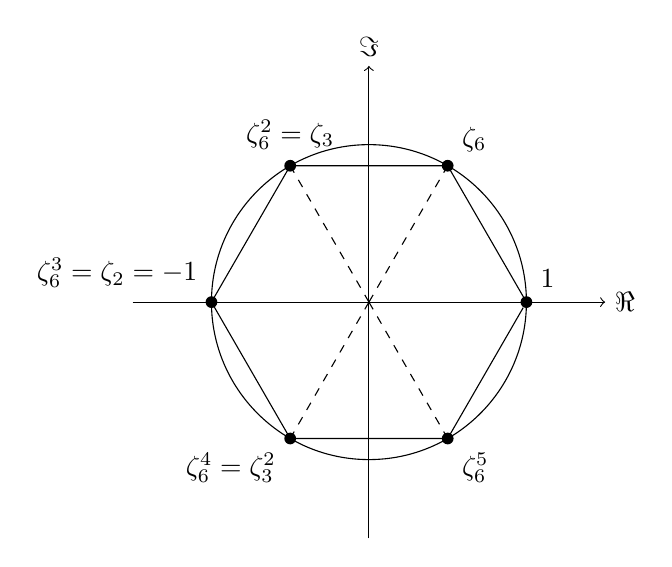
\begin{tikzpicture}[x=2cm,y=2cm]
      \draw (0,0) circle (1);

      \draw (0:1) node[circle,fill,inner sep=1.5pt, label=above right:$1$] (m0) {} --
      (60:1) node[circle,fill,inner sep=1.5pt, label=above right:$\zeta_6$] (m1) {} --
      (120:1) node[circle,fill,inner sep=1.5pt, label=above:{$\zeta_6^2 = \zeta_3$}] (m2) {} --
      (180:1) node[circle,fill,inner sep=1.5pt, label=above left:{$\zeta_6^3 = \zeta_2 = -1$}] (m3) {} --
      (240:1) node[circle,fill,inner sep=1.5pt, label=below left:{$\zeta_6^4 = \zeta_3^2$}] (m4) {} --
      (300:1) node[circle,fill,inner sep=1.5pt, label=below right:{$\zeta_6^5$}] (m5) {} -- (m0);

      \draw[dashed] (0,0) -- (60:1);
      \draw[dashed] (0,0) -- (120:1);
      \draw[dashed] (0,0) -- (240:1);
      \draw[dashed] (0,0) -- (300:1);

      \draw[->] (-1.5,0) -- (+1.5,0) node[right] {$\Re$};
      \draw[->] (0,-1.5) -- (0,+1.5) node[above] {$\Im$};
    \end{tikzpicture}
  \end{center}
  \caption{Las raíces sextas de la unidad en el plano complejo}
\end{figure}

Notamos un par de propiedades.

\begin{enumerate}
\item[1)] Si $m \mid n$, entonces toda raíz $m$-ésima es una raíz $n$-ésima.

  Esto se ve de la identidad $z^n = (z^m)^{n/m}$ o también de
  $\zeta_m = \zeta_n^{n/m}$.

\item[2)] Para cualquier $n \ge 2$ la suma de todas las raíces $n$-ésimas es
  nula:
  $$1 + \zeta_n + \zeta_n^2 + \cdots + \zeta_n^{n-1} = \frac{\zeta_n^n-1}{\zeta_n-1} = 0$$
  ---aquí hemos usado la fórmula para la serie geométrica y el hecho de que
  $\zeta_n \ne 1$.
\end{enumerate}

% % % % % % % % % % % % % % % % % % % % % % % % % % % % % %

\section{Axiomas de anillos}

Hasta el momento hemos revisado las construcciones de los números racionales
$\QQ$, reales $\RR$ y complejos $\CC$. Cada uno de estos conjuntos está formado
por ciertos elementos, sobre cuáles están definidas la suma y producto que
cumplen las propiedades habituales enumeradas en
\ref{obs:los-complejos-forman-un-anillo}. De la misma manera, sobre el conjunto
$\ZZ/n\ZZ$ de los restos módulo $n$ están definidas las dos operaciones
aritméticas. Para generalizar y axiomatizar todos estos ``conjuntos de
números'', se introduce la noción de \term{anillo}.

\begin{definicion}
  Un \term{anillo} $A$ es un conjunto dotado de dos
  operaciones: \term{adición}
  \begin{align*}
    +\colon A\times A & \to A,\\
    (x,y) & \mapsto x+y
  \end{align*}
  y \term{multiplicación}
  \begin{align*}
    \cdot\colon A\times A & \to A,\\
    (x,y) & \mapsto xy
  \end{align*}
  que satisfacen los siguientes axiomas.

  \begin{enumerate}
  \item[A1a)] la adición es \term{asociativa}: para cualesquiera $x,y,z\in A$
    tenemos
    $$(x+y)+z = x+(y+z);$$

  \item[A1b)] existe un elemento $0\in A$ (el \term{cero}) tal que para todo
    $x\in A$ se cumple
    $$0+x = x = x+0;$$

  \item[A1c)] para todo $x\in A$ existe un elemento $-x\in A$ (el \term{opuesto}
    de $x$) que satisface
    $$(-x) + x = x + (-x) = 0;$$

  \item[A1d)] la adición es \term{conmutativa}: para cualesquiera $x,y\in A$ se
    cumple
    $$x+y = y+x;$$

  \item[A2)] la multiplicación es \term{distributiva}
    respecto a la adición: para cualesquiera $x,y,z\in A$ se cumple
    $$x\,(y+z) = xy + xz, \quad (x+y)\,z = xz + yz;$$

  \item[A3)] la multiplicación es \term{asociativa}: para cualesquiera
    $x,y,z\in A$ tenemos
    $$(xy)\,z = x\,(yz);$$

  \item[A4)] existe un elemento $1\in A$ (la \term{identidad}) tal que para todo
    $x\in A$ se cumple
    $$1\cdot x = x = x\cdot 1.$$
  \end{enumerate}
  Además, si se cumple el axioma adicional
  \begin{enumerate}
  \item[AC)] la multiplicación es \term{conmutativa}: para cualesquiera
    $x,y\in A$ se cumple
    $$xy = yx.$$
  \end{enumerate}
  se dice que $A$ es un \term{anillo conmutativo}.
\end{definicion}

% % % % % % % % % % % % % % % % % % % % % % % % % % % % % %

\section{Ejemplos de anillos}

\begin{ejemplo}
  Al revisar los axiomas, no debe ser sorprendente que los números enteros
  $\ZZ$, racionales $\QQ$, reales $\RR$, complejos $\CC$ formen anillos
  conmutativos respecto a la adición y multiplicación habitual.
\end{ejemplo}

\begin{ejemplo}
  \label{ejemplo:anillo-ZnZ}
  Para $n = 1, 2, 3, \ldots$ hemos notado en el capítulo 0 que sobre el conjunto
  $$\ZZ/n\ZZ \dfn \{ [a]_n \mid a \in \ZZ \} = \{ [0]_n, [1]_n, \ldots, [n-1]_n \}$$
  formado por los restos módulo $n$
  $$[a]_n \dfn \{ b\in \ZZ \mid a\equiv b \pmod{n} \}$$
  se puede definir la adición y multiplicación mediante las fórmulas
  \begin{align*}
    [a]_n + [b]_n & \dfn [a+b]_n,\\
    [a]_n \cdot [b]_n & \dfn [ab]_n.
  \end{align*}

  Se ve que $\ZZ/n\ZZ$ es un anillo conmutativo respecto a la adición y
  multiplicación módulo $n$, dado que $\ZZ$ lo es. Los restos $[0]_n$ y $[1]_n$
  son el cero y la identidad respectivamente. Los elementos opuestos son dados
  por $-[a]_n = [-a]_n$.
\end{ejemplo}

Un ejemplo extremadamente importante son los anillos de polinomios.

\begin{ejemplo}[Anillos de polinomios]
  Sea $A$ un anillo. Un \term{polinomio} con coeficientes en
  $A$ en una variable $X$ es una \term{suma formal}
  $$f = \sum_{i\ge 0} a_i\,X^i,$$
  donde $a_i \in A$, y casi todos los $a_i$ son nulos, excepto un número finito
  de ellos. Esto quiere decir que la suma formal de arriba es finita: para algún
  $n$ tenemos
  \begin{equation}
    \label{eqn:polinomio-expresion-finita}
    f = \sum_{0 \le i\le n} a_i\,X^i =  a_n\,X^n + a_{n-1}\,X^{n-1} + \cdots + a_1\,X + a_0.
  \end{equation}

  La palabra ``suma formal'' significa que
  $\sum_{i\ge 0} a_i\,X^i = \sum_{i\ge 0} b_i\,X^i$ si y solo si $a_i = b_i$
  para todo $i \ge 0$. Para denotar las variables de polinomios, serán usadas
  las letras mayúsculas $X,Y,Z,\ldots$ Los términos de la forma $0\cdot X^i$
  normalmente se omiten de las expresiones como
  \eqnref{eqn:polinomio-expresion-finita}.

  Las sumas de polinomios están definidas término por término:
  $$\sum_{i\ge 0} a_i\,X^i + \sum_{i\ge 0} b_i\,X^i \dfn \sum_{i\ge 0} (a_i + b_i)\,X^i.$$

  Para definir los productos, basta declarar que los monomios se multiplican
  como
  $$a_i\,X^i \cdot b_j\,X^j = a_i b_j \, X^{i+j},$$
  y aplicar la distributividad:
  \begin{multline*}
    \left(a_m\,X^m + a_{m-1}\,X^{m-1} + \cdots + a_1\,X + a_0\right) \, \left(b_n\,X^n + b_{n-1}\,X^{n-1} + \cdots + b_1\,X + b_0\right) \\
    = a_m b_n\,X^{m+n} + (a_m\,b_{n-1} + a_{m-1}\,b_n)\,X^{m+n-1} + \cdots + (a_1 b_0 + a_0 b_1)\,X + a_0 b_0.
  \end{multline*}
  Esto nos lleva a la fórmula
  \[ \left(\sum_{i\ge 0} a_i\,X^i\right) \cdot \left(\sum_{i\ge 0} b_i\,X^i\right) \dfn
  \sum_{k\ge 0} \left(\sum_{i+j = k} a_i b_j\right)\,X^k. \]

  Dejo al lector verificar que los polinomios forman un anillo respecto a estas
  operaciones. Este anillo se denotará por $A [X]$. Notamos que si $A$ es
  conmutativo, entonces $A [X]$ es también conmutativo (este es el caso que nos
  va a interesar a continuación). Tal vez la parte menos evidente es la
  asociatividad de multiplicación. Para probarla, se puede observar que si
  \[ f = \sum_{i\ge 0} a_i\,X^i, \quad
  g = \sum_{j\ge 0} b_j\,X^j, \quad
  h = \sum_{k\ge 0} c_k\,X^k, \]
  entonces ambas expresiones $f\,(g \, h)$ y $(f \, g)\,h$ son iguales a
  $$\sum_{n\ge 0} \left(\sum_{i+j+k = n} a_i b_j c_k\right)\,X^n.$$

  Un polinomio de la forma
  $$c + 0\cdot X + 0\cdot X^2 + 0\cdot X^3 + \cdots$$
  se llama un \term{polinomio constante} y también se denota por $c$. El cero en
  $A [X]$ es el polinomio constante $0$ y la identidad es el polinomio constante
  $1$.

  Si seguimos la misma construcción, pero quitamos la condición de que
  $a_i = 0$, excepto un número finito de $i$, entonces se obtiene el
  \term{anillo de las series formales} que se denota por $A[\![X]\!]$. Véase el
  ejercicio \ref{ejerc:series-formales}.
\end{ejemplo}

Vamos a volver a los polinomios en el siguiente capítulo para sistematizar sus
propiedades.

\begin{ejemplo}[Anillos de funciones]
  Sea $X$ un conjunto y $A$ un anillo. Las aplicaciones $f\colon X\to A$ forman
  un anillo respecto a la suma y producto \term{punto por punto}:
  $$(f+g) (x) \dfn f (x) + g (x), \quad (fg) (x) \dfn f (x) \, g (x).$$
  Los axiomas de anillos se deducen de estos axiomas para $A$. El cero es
  la aplicación constante $x \mapsto 0$ y la identidad es la aplicación
  constante $x \mapsto 1$. Este anillo se llama el
  \term{anillo de funciones sobre $X$} con valores en $A$ y se denotará por
  $\Fun (X,A)$. Si $A$ es un anillo conmutativo, entonces el anilo $\Fun (X,A)$
  es también conmutativo.

  Los anillos de funciones tienen mucha importancia en la geometría moderna,
  donde $X$ es algún espacio geométrico y la idea principal es reconstruir $X$ a
  partir de las funciones sobre $X$.
\end{ejemplo}

Mencionemos un ejemplo importante de anillos no conmutativos que seguramente es
familiar al lector.

\begin{ejemplo}[Anillos de matrices]
  Para un anillo $A$, una \term{matriz de $n\times n$ con coeficientes en $A$}
  es una tabla
  \[ a = \begin{pmatrix}
      a_{11} & a_{12} & \cdots & a_{1n} \\
      a_{21} & a_{22} & \cdots & a_{2n} \\
      \vdots & \vdots & \ddots & \vdots \\
      a_{n1} & a_{n2} & \cdots & a_{nn} \\
    \end{pmatrix} \]
  donde $a_{ij} \in A$. En este curso vamos a denotar las matrices nada más por
  las letras minúsculas $a, b, c, \ldots$ La suma de matrices se define término
  por término:
  \[ \begin{pmatrix}
      a_{11} & \cdots & a_{1n} \\
      \vdots & \ddots & \vdots \\
      a_{n1} & \cdots & a_{nn} \\
    \end{pmatrix} +
    \begin{pmatrix}
      b_{11} & \cdots & b_{1n} \\
      \vdots & \ddots & \vdots \\
      b_{n1} & \cdots & b_{nn} \\
    \end{pmatrix} \dfn
    \begin{pmatrix}
      a_{11} + b_{11} & \cdots & a_{1n} + b_{1n} \\
      \vdots & \ddots & \vdots \\
      a_{n1} + b_{n1} & \cdots & a_{nn} + b_{nn} \\
    \end{pmatrix}, \]
  mientras que el producto
  \[ \begin{pmatrix}
      a_{11} & \cdots & a_{1n} \\
      \vdots & \ddots & \vdots \\
      a_{n1} & \cdots & a_{nn} \\
    \end{pmatrix} \cdot \begin{pmatrix}
      b_{11} & \cdots & b_{1n} \\
      \vdots & \ddots & \vdots \\
      b_{n1} & \cdots & b_{nn} \\
    \end{pmatrix} =
    \begin{pmatrix}
      c_{11} & \cdots & c_{1n} \\
      \vdots & \ddots & \vdots \\
      c_{n1} & \cdots & c_{nn} \\
    \end{pmatrix} \]
  se define mediante la fórmula
  $$c_{ij} \dfn \sum_{1 \le k \le n} a_{ik}\,b_{kj}.$$
  Este producto no es algo aleatorio: su definición viene de la composición de
  aplicaciones lineales.

  Las matrices de $n\times n$ con coeficientes en $A$ forman un anillo que vamos
  a denotar por $M_n (A)$. El cero es la matriz nula
  \[ 0 \dfn \begin{pmatrix}
      0 & 0 & \cdots & 0 \\
      0 & 0 & \cdots & 0 \\
      \vdots & \vdots & \ddots & \vdots \\
      0 & 0 & \cdots & 0 \\
    \end{pmatrix} \]
  y la identidad es la matriz
  \[ 1 \dfn \begin{pmatrix}
      1 & 0 & \cdots & 0 \\
      0 & 1 & \cdots & 0 \\
      \vdots & \vdots & \ddots & \vdots \\
      0 & 0 & \cdots & 1 \\
    \end{pmatrix}. \]
  En un primer curso de álgebra lineal normalmente se considera $A = \RR$ o
  $\CC$ y se verifican los axiomas de anillos para este caso, pero el anillo
  específico $A$ es irrelevante para llevar a cabo la construcción general.

  El anillo $M_n (A)$ no es conmutativo para $n \ge 2$: por ejemplo, para
  $n = 2$ podemos considerar las matrices
  \[ e_{11} \dfn \begin{pmatrix}
      1 & 0 \\
      0 & 0
    \end{pmatrix}, \quad
    e_{12} \dfn \begin{pmatrix}
      0 & 1 \\
      0 & 0
    \end{pmatrix}. \]
  Calculamos que
  $$e_{11}\,e_{12} = e_{12}, \quad e_{12}\,e_{11} = 0,$$
  y luego $e_{11}\,e_{12} \ne e_{12}\,e_{11}$, salvo el caso trivial cuando en
  $A$ se cumple $1 = 0$.
\end{ejemplo}

No olvidemos que las matrices sirven nada más para especificar las aplicaciones
lineales $V\to V$ respecto a una base fija de $V$. Sin fijar una base, podemos
definir de manera abstracta el anillo de aplicaciones lineales.

\begin{ejemplo}
  Para un espacio vectorial $V$, sea $\End (V)$ el conjunto de las aplicaciones
  lineales $f\colon V\to V$. Definamos la suma mediante
  $$(f+g) (v) \dfn f (v) + g (v)$$
  y el producto mediante la composición de aplicaciones $f\circ g$. Esto nos da
  una estructura de anillo no conmutativo sobre $\End (V)$ que se llama
  el \term{anillo de endomorfismos} de $V$.
\end{ejemplo}

\begin{ejemplo}
  Una manera común de construir nuevos anillos es tomar productos. A saber, para
  dos anillos $A$ y $B$, el \term{producto} $A\times B$ se define como
  el producto cartesiano respecto a las operaciones
  \[ (a_1,b_1) + (a_2,b_2) \dfn (a_1+a_2, b_1+b_2), \quad
    (a_1,b_1) \cdot (a_2,b_2) \dfn (a_1 a_2, b_1 b_2). \]
  Dejo al lector verificar que $A\times B$ es un anillo. Si $A$ y $B$ son
  conmutativos, entonces $A\times B$ es también conmutativo.

  De la misma manera, para una familia de anillos $A_i$, el producto
  $\prod_{i\in I} A_i$ se define como el producto cartesiano respecto a las
  operaciones
  \[ (a_i)_i + (a_i')_i \dfn (a_i+a_i')_i, \quad
    (a_i)_i \cdot (a_i')_i \dfn (a_i a_i')_i. \qedhere \]
\end{ejemplo}

% % % % % % % % % % % % % % % % % % % % % % % % % % % % % %

\section{Algunos no-anillos ($\clubsuit$)}

Sería instructivo considerar algo parecido a anillo que no cumpla algún axioma
de la lista.

\begin{ejemplo}
  Para los polinomios
  $$f = \sum_{i\ge 0} a_i\,X^i, ~ g = \sum_{i\ge 0} b_i\,X^i \in A [X]$$
  tomemos la suma habitual y el producto dado por la sustitución
  $$f \circ g \dfn f (g (X)) \dfn \sum_{k\ge 0} a_k\,\left(\sum_{i\ge 0} b_i\,X^i\right)^k.$$

  Notamos que
  $$(f_1 + f_2)\circ g = f_1\circ g + f_2\circ g,$$
  pero en general
  $$f\circ (g_1 + g_2) \ne f_1\circ g_1 + f_1\circ g_2.$$
  Por ejemplo, si $f = X^2$, $g_1 = X$, $g_2 = 1$, entonces
  $$f\circ (g_1 + g_2) = X^2 + 2X + 1, \text{ mientras que } f\circ g_1 + f\circ g_2 = X^2 + 1.$$
  Estas dos expresiones no coinciden si $2 \ne 0$ en $A$. Este ejemplo demuestra
  la importancia de tener en el caso no conmutativo dos condiciones de
  distributividad: por la izquierda y por la derecha.
\end{ejemplo}

\begin{ejemplo}
  Recordemos que sobre el espacio $\RR^3$ se puede definir el
  \term{producto cruz}
  $$\times\colon \RR^3\times \RR^3 \to \RR^3$$
  mediante
  \[ u \times v \dfn
    \left|\begin{array}{ccc}
            \vec{e}_1 & \vec{e}_2 & \vec{e}_3 \\
            u_1 & u_2 & u_3 \\
            v_1 & v_2 & v_3\end{array}\right| \dfn
     \left|\begin{array}{cc}
             u_2 & u_3 \\
             v_2 & v_3
           \end{array}\right|\,\vec{e}_1
     - \left|\begin{array}{cc}
                      u_1 & u_3 \\
                      v_1 & v_3
                \end{array}\right|\,\vec{e}_2
      + \left|\begin{array}{cc}
                u_1 & u_2 \\
                v_1 & v_2
              \end{array}\right|\,\vec{e}_3, \]
  donde
  \begin{gather*}
    \vec{e}_1 \dfn (1,0,0), ~
    \vec{e}_2 \dfn (0,1,0), ~
    \vec{e}_3 \dfn (0,0,1);\\
    u = (u_1, u_2, u_3), \quad
    v = (v_1, v_2, v_3).
  \end{gather*}
  El lector puede verificar que el producto cruz es distributivo respecto a la
  adición habitual de vectores:
  \[ u\times (v + w) = u\times v + u\times w, \quad
    (u + v)\times w = u\times w + v\times w. \]
  Notamos que para cualquier $u \in \RR^3$ se cumple
  $$u \times u = \vec{0}.$$
  En particular, tenemos
  $$(u + v) \times (u + v) = \underbrace{u\times u}_{=\vec{0}} + u\times v + v\times u + \underbrace{v\times v}_{=\vec{0}},$$
  así que
  $$v\times u = -u\times v.$$
  Esto significa que se tiene una especie de anillo no conmutativo. Sin embargo,
  hay dos problemas.

  \begin{itemize}
  \item[1)] Primero, falta la identidad: esta tendría que cumplir
    $\vec{1}\times\vec{1} = \vec{1}$, pero $\vec{1}\times\vec{1} = \vec{0}$, y
    el vector nulo $\vec{0}$ claramente no funciona como la identidad.

  \item[2)] El producto cruz no es asociativo: en general
    $$(u\times v)\times w \ne u\times (v\times w),$$
    y en lugar de la asociatividad se cumple la \term{identidad de Jacobi}
    $$u \times (v \times w) + v \times (w \times u) + w \times (u \times  v) = 0.$$

    \ifwordy
    \begin{shaded}
      Por ejemplo, los vectores de la base se multiplican de la siguiente
      manera:

      \begin{center}
        \begin{tabular}{x{1cm}|x{1cm}x{1cm}x{1cm}}
          $\times$ & $\vec{e}_1$ & $\vec{e}_2$ & $\vec{e}_3$ \tabularnewline
          \hline
          $\vec{e}_1$ & $\mathbf{0}$ & $\vec{e}_3$ & $-\vec{e}_2$ \tabularnewline
          $\vec{e}_2$ & $-\vec{e}_3$ & $\mathbf{0}$ & $\vec{e}_1$ \tabularnewline
          $\vec{e}_3$ & $\vec{e}_2$ & $-\vec{e}_1$ & $\mathbf{0}$ \tabularnewline
        \end{tabular}
      \end{center}
      Así que
      $$(\vec{e}_1 \times \vec{e}_2)\times \vec{e}_2 = \vec{e}_3\times \vec{e}_2 = -\vec{e}_1,$$
      mientras que
      $$\vec{e}_1 \times (\vec{e}_2\times \vec{e}_2) = \vec{e}_1\times \mathbf{0} = \mathbf{0}.$$
    \end{shaded}
    \fi
  \end{itemize}

  Usando el producto cruz, se puede definir una estructura de anillo no sobre
  $\RR^3$, sino sobre $\RR^4$. Identifiquemos los elementos de $\RR^4$ con pares
  $(a,u)$, donde $a \in \RR$ y $u \in \RR^3$. Las operaciones
  \begin{align*}
    (a,u) + (b,v) & \dfn (a+b, u+v),\\
    (a,u) \cdot (b,v) & \dfn (ab - u\cdot v, \, av + bu + u\times v).
  \end{align*}
  definen un anillo no conmutativo que se conoce como el
  \term{anillo de cuaterniones} y se denota por $\HH$\footnote{La letra $\HH$
    conmemora al descubridor de cuaterniones, el matemático irlandés
    \personality{William Rowan Hamilton} (1805--1865).}. Véase el ejercicio
  \ref{ejerc:cuaterniones}.
\end{ejemplo}

\begin{ejemplo}
  He aquí otro ejemplo parecido: para dos matrices $a,b \in M_n (A)$ definamos
  su \term{conmutador} como la matriz
  \begin{equation}
    \label{eqn:conmutador-de-matrices}
    [a,b] \dfn ab - ba.
  \end{equation}
  Notamos que $[a,b] = 0$ si y solo si las matrices conmutan: $ab = ba$. Tenemos
  $[a,a] = 0$ y $[a,b] = - [b,a]$. En general,
  $$[[a,b],c] \ne [a,[b,c]],$$
  pero para cualesquiera $a,b,c\in M_n (A)$ se cumple la identidad de Jacobi
  $$[a,[b,c]] + [b,[c,a]] + [c,[a,b]] = 0$$
  ---dejo al lector el placer de desarrollar los corchetes según la definición
  \eqnref{eqn:conmutador-de-matrices} y verificar que todos los términos se
  cancelan.
\end{ejemplo}

Para nosotros, el término ``anillo'' siempre asume la existencia de identidad y
la asociatividad del producto, así que $\RR^3$ con el producto cruz y las
matrices con el conmutador $[-,-]$ no son anillos. Son casos particulares de
algo llamado ``anillos de Lie\footnote{\personality{Sophus Lie} (1842--1899),
  matemático noruego, conocido por sus trabajos en la teoría de grupos de
  Lie.}'', que es también una estructura sumamente importante, pero no la vamos
a estudiar en este curso.

% % % % % % % % % % % % % % % % % % % % % % % % % % % % % %

\section{Subanillos}

Si tenemos un anillo $A$ y un subconjunto $B \subseteq A$, para asegurarnos que
$B$ es también un anillo respecto a la misma suma y producto, basta verificar
que $B$ contiene $0$ y $1$ y que las operaciones $(x,y)\mapsto x+y$,
$x\mapsto -x$, $(x,y) \mapsto xy$ se restringen a $B$. Esto nos lleva a
la noción de subanillo.

\begin{definicion}
  Sea $A$ un anillo. Se dice que un subconjunto $B \subseteq A$ es un
  \term{subanillo} de $A$ si

  \begin{enumerate}
  \item[1)] $B$ es cerrado respecto a la adición y elementos opuestos:

    \begin{itemize}
    \item[a)] $0 \in B$,
    \item[b)] $x+y \in B$ para cualesquiera $x,y\in B$,
    \item[c)] $-x \in B$ para todo $x\in B$;
    \end{itemize}

  \item[2)] $B$ es cerrado respecto a la multiplicación:

    \begin{itemize}
    \item[a)] $1 \in B$,
    \item[b)] $xy\in B$ para cualesquiera $x,y\in B$.
    \end{itemize}
  \end{enumerate}
\end{definicion}

El lector puede comprobar que en este caso $B$ es también un anillo respecto
a las mismas operaciones que $A$.

\begin{observacionejerc}
  Sea $A$ un anillo. Si $A_i \subseteq A$ son subanillos, entonces
  $\bigcap_i A_i$ es un subanillo.
\end{observacionejerc}

\begin{ejemplo}
  Tenemos una cadena de subanillos
  \[ \ZZ \subset \QQ \subset \RR \subset \CC. \qedhere \]
\end{ejemplo}

\begin{ejemplo}
  Los números naturales $\NN$ no forman un subanillo de $\ZZ$: si $n \in \NN$,
  entonces $-n \notin \NN$, salvo cuando $n = 0$.
\end{ejemplo}

\begin{ejemplo}
  Las matrices de la forma
  \[ \begin{pmatrix}
      x & 0 \\
      0 & 0
    \end{pmatrix}, \quad x\in A \]
  cumplen todas las condiciones, salvo que la matriz identidad no está entre
  ellas. Entonces, tales matrices no forman un subanillo de $M_2 (A)$ según
  nuestra definición de arriba.
\end{ejemplo}

\begin{ejemplo}
  El \term{anillo de los enteros de Gauss}\footnote{\personality{Carl Friedrich
      Gauss} (1777--1855) --- matemático alemán. Entre otras cosas, escribió a
    los veintiún años su tratado ``Disquisitiones arithmeticae'' que revolucionó
    el área de la teoría de números.}  es dado por
  $$\ZZ [i] \dfn \{ a + bi \mid a,b \in \ZZ \} \subset \CC,$$
  Se ve fácilmente que este es un subanillo de $\CC$.
\end{ejemplo}

\begin{figure}[h]
  \begin{center}
    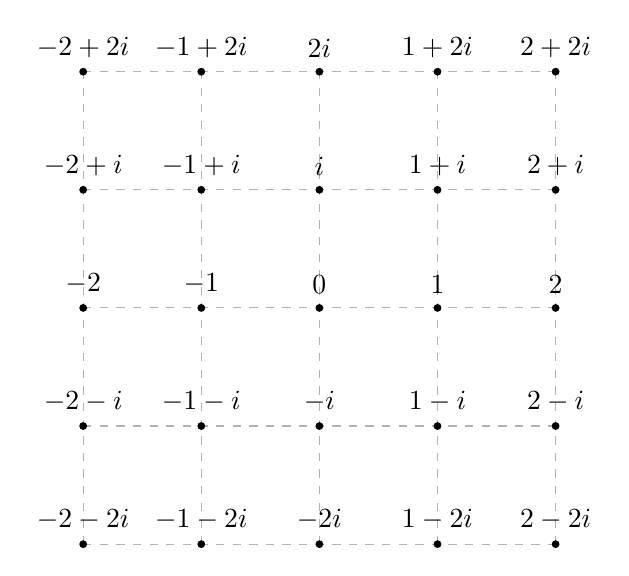
\begin{tikzpicture}[x=1.5cm, y=1.5cm]

      \foreach \i in {-2,...,2}
      \draw[black!30,dashed] (\i,-2) -- (\i,2);

      \foreach \j in {-2,...,2}
      \draw[black!30,dashed] (-2,\j) -- (2,\j);

      \draw (-2,0) node[circle,fill,inner sep=1pt, label=above:{$-2$}] {};
      \draw (-1,0) node[circle,fill,inner sep=1pt, label=above:{$-1$}] {};
      \draw (0,0) node[circle,fill,inner sep=1pt, label=above:{$0$}] {};
      \draw (1,0) node[circle,fill,inner sep=1pt, label=above:{$1$}] {};
      \draw (2,0) node[circle,fill,inner sep=1pt, label=above:{$2$}] {};

      \draw (-2,1) node[circle,fill,inner sep=1pt, label=above:{$-2+i$}] {};
      \draw (-1,1) node[circle,fill,inner sep=1pt, label=above:{$-1+i$}] {};
      \draw (0,1) node[circle,fill,inner sep=1pt, label=above:{$i$}] {};
      \draw (1,1) node[circle,fill,inner sep=1pt, label=above:{$1+i$}] {};
      \draw (2,1) node[circle,fill,inner sep=1pt, label=above:{$2+i$}] {};

      \draw (-2,-1) node[circle,fill,inner sep=1pt, label=above:{$-2-i$}] {};
      \draw (-1,-1) node[circle,fill,inner sep=1pt, label=above:{$-1-i$}] {};
      \draw (0,-1) node[circle,fill,inner sep=1pt, label=above:{$-i$}] {};
      \draw (1,-1) node[circle,fill,inner sep=1pt, label=above:{$1-i$}] {};
      \draw (2,-1) node[circle,fill,inner sep=1pt, label=above:{$2-i$}] {};

      \draw (-2,2) node[circle,fill,inner sep=1pt, label=above:{$-2+2i$}] {};
      \draw (-1,2) node[circle,fill,inner sep=1pt, label=above:{$-1+2i$}] {};
      \draw (0,2) node[circle,fill,inner sep=1pt, label=above:{$2i$}] {};
      \draw (1,2) node[circle,fill,inner sep=1pt, label=above:{$1+2i$}] {};
      \draw (2,2) node[circle,fill,inner sep=1pt, label=above:{$2+2i$}] {};

      \draw (-2,-2) node[circle,fill,inner sep=1pt, label=above:{$-2-2i$}] {};
      \draw (-1,-2) node[circle,fill,inner sep=1pt, label=above:{$-1-2i$}] {};
      \draw (0,-2) node[circle,fill,inner sep=1pt, label=above:{$-2i$}] {};
      \draw (1,-2) node[circle,fill,inner sep=1pt, label=above:{$1-2i$}] {};
      \draw (2,-2) node[circle,fill,inner sep=1pt, label=above:{$2-2i$}] {};
    \end{tikzpicture}
  \end{center}

  \caption{Los enteros de Gauss $\ZZ [i]$ en el plano complejo}
\end{figure}

\begin{ejemplo}
  \label{ejemplo:enteros-de-eisenstein}
  Otro ejemplo del mismo tipo: consideremos la raíz cúbica de la unidad
  $\zeta_3 \dfn e^{2\pi i/3}$ y el conjunto
  $$\ZZ [\zeta_3] \dfn \{ a + b\,\zeta_3 \mid a,b \in \ZZ \} \subset \CC.$$
  Está claro que para cualesquiera $x,y \in \ZZ [\zeta_3]$ se tiene
  $x+y \in \ZZ [\zeta_3]$. Para la multiplicación, caculamos que
  $$(a + b\,\zeta_3)\cdot (c + d\,\zeta_3) = ac + (ad + bc)\,\zeta_3 + bd\,\zeta_3^2,$$
  y usando la relación $\zeta_3^2 = -1 - \zeta_3$, podemos escribir la última
  expresión como
  $$(ac - bd) + (ad + bc - bd)\,\zeta_3 \in \ZZ [\zeta_3].$$
  Después de esta verificación se ve que $\ZZ [\zeta_3]$ es un subanillo de
  $\CC$. Este se llama el \term{anillo de los enteros de
    Eisenstein}\footnote{\personality{Ferdinand Gotthold Max Eisenstein}
    (1823--1852), matemático alemán, estudiante de Dirichlet, conocido por sus
    contribuciones en la teoría de números. Murió a los 29 años de
    tuberculosis.}.
\end{ejemplo}

\begin{figure}[h]
  \begin{center}
    \begin{tikzpicture}[x=1.7cm, y=1.7cm]
      \draw ({cos(0)},{sin(0)}) coordinate (x);
      \draw ({cos(60)},{sin(60)}) coordinate (y);

      \draw[black!30,dashed] ($-2*(x)+2*(y)$) -- ($2*(x)-2*(y)$);
      \draw[black!30,dashed] ($2*(y)$) -- ($-2*(y)$);
      \draw[black!30,dashed] ($2*(x)$) -- ($-2*(x)$);
      \draw[black!30,dashed] ($-2*(x)+2*(y)$) -- ($-2*(x)$);
      \draw[black!30,dashed] ($-1*(x)+2*(y)$) -- ($-1*(x) + -1*(y)$);
      \draw[black!30,dashed] ($2*(x)-2*(y)$) -- ($2*(x)$);
      \draw[black!30,dashed] ($(x)-2*(y)$) -- ($(x) + (y)$);
      \draw[black!30,dashed] ($-2*(x)+2*(y)$) -- ($2*(y)$);
      \draw[black!30,dashed] ($-2*(x)+(y)$) -- ($(x) + (y)$);
      \draw[black!30,dashed] ($-1*(x) + -1*(y)$) -- ($2*(x)-(y)$);
      \draw[black!30,dashed] ($-2*(y)$) -- ($2*(x)-2*(y)$);
      \draw[black!30,dashed] ($2*(y)$) -- ($2*(x)$);
      \draw[black!30,dashed] ($-1*(x)+2*(y)$) -- ($2*(x)-(y)$);
      \draw[black!30,dashed] ($-2*(y)$) -- ($-2*(x)$);
      \draw[black!30,dashed] ($(x)-2*(y)$) -- ($-2*(x)+(y)$);

      \draw (0,0) node[circle,fill,inner sep=1pt, label=above:{$0$}] {};

      \draw (x) node[circle,fill,inner sep=1pt, label=above:{$1$}] {};
      \draw (y) node[circle,fill,inner sep=1pt, label=above:{$1+\zeta_3$}] {};
      \draw ($-1*(x)+(y)$) node[circle,fill,inner sep=1pt, label=above:{$\zeta_3$}] {};
      \draw ($-1*(x)$) node[circle,fill,inner sep=1pt, label=above:{$-1$}] {};
      \draw ($-1*(y)$) node[circle,fill,inner sep=1pt, label=above:{$-1-\zeta_3$}] {};
      \draw ($(x)-(y)$) node[circle,fill,inner sep=1pt, label=above:{$-\zeta_3$}] {};

      \draw ($(x) + (y)$) node[circle,fill,inner sep=1pt, label=above:{$2+\zeta_3$}] {};
      \draw ($-1*(x)+2*(y)$) node[circle,fill,inner sep=1pt, label=above:{$1+2\,\zeta_3$}] {};
      \draw ($-2*(x)+(y)$) node[circle,fill,inner sep=1pt, label=above:{$-1+\zeta_3$}] {};
      \draw ($-1*(x) + -1*(y)$) node[circle,fill,inner sep=1pt, label=above:{$-2-\zeta_3$}] {};
      \draw ($(x)-2*(y)$) node[circle,fill,inner sep=1pt, label=above:{$1-2\,\zeta_3$}] {};
      \draw ($2*(x)-(y)$) node[circle,fill,inner sep=1pt, label=above:{$1-\zeta_3$}] {};

      \draw ($2*(x)$) node[circle,fill,inner sep=1pt, label=above:{ $2$}] {};
      \draw ($2*(y)$) node[circle,fill,inner sep=1pt, label=above:{$2+2\,\zeta_3$}] {};
      \draw ($-2*(x)+2*(y)$) node[circle,fill,inner sep=1pt, label=above:{$2\,\zeta_3$}] {};
      \draw ($-2*(x)$) node[circle,fill,inner sep=1pt, label=above:{$-2$}] {};
      \draw ($-2*(y)$) node[circle,fill,inner sep=1pt, label=above:{$-2-2\,\zeta_3$}] {};
      \draw ($2*(x)-2*(y)$) node[circle,fill,inner sep=1pt, label=above:{$-2\,\zeta_3$}] {};
    \end{tikzpicture}
  \end{center}
  \caption{Los enteros de Eisenstein $\ZZ [\zeta_3]$ en el plano complejo}
\end{figure}

\begin{ejemplo}
  Sea $n \ne 1$ un entero libre de cuadrados\footnote{Es decir, $p^2 \nmid n$
    para ningún primo $p$. Los primeros números libres de cuadrados son
    $$\pm 1, \pm 2, \pm 3, \pm 5, \pm 6, \pm 7, \pm 10, \pm 11, \pm 13, \pm 14, \pm 15, \pm 17, \ldots$$}. Pongamos
  $$\QQ (\sqrt{n}) \dfn \{ a + b\sqrt{n} \mid a,b\in \QQ \}.$$
  Este es un subanillo de $\RR$ si $n > 0$ y un subanillo de $\CC$ si
  $n < 0$. Por ejemplo, calculemos los productos:
  $$(a+b\sqrt{n}) \, (c+d\sqrt{n}) = ac + n\,bd + (ad+bc)\,\sqrt{n}.$$
  Por las mismas consideraciones, el conjunto
  $$\ZZ [\sqrt{n}] \dfn \{ a + b\sqrt{n} \mid a,b\in \ZZ \}$$
  es un subanillo de $\QQ (\sqrt{n})$.

  En el caso cuando $n \equiv 1 \pmod{4}$, se puede considerar el conjunto más
  grande
  \[ \ZZ \Bigl[\frac{1+\sqrt{n}}{2}\Bigr] \dfn
    \Bigl\{ a + b\,\frac{1+\sqrt{n}}{2} \Bigm| a,b\in \ZZ \Bigr\}. \]
  Este es también un subanillo de $\QQ (\sqrt{n})$. La parte menos evidente son
  los productos:
  \[ \left(a + b\,\frac{1+\sqrt{n}}{2}\right)\,\left(c + d\,\frac{1+\sqrt{n}}{2}\right) =
    ac + bd\,\frac{1 + 2\sqrt{n} + n}{4} + (ad + bc)\,\frac{1+\sqrt{n}}{2}. \]
  Ahora ya que $n = 4k + 1$ para algún $k \in \ZZ$,
  $$\frac{1 + 2\sqrt{n} + n}{4} = \frac{1 + \sqrt{n}}{2} + k,$$
  así que el producto pertenece a $\ZZ \Bigl[\frac{1+\sqrt{n}}{2}\Bigr]$. 

  Tenemos una cadena de subanillos
  \[ \ZZ \subset \ZZ [\sqrt{n}] \subset
    \ZZ \Bigl[\frac{1+\sqrt{n}}{2}\Bigr] \subset
    \QQ (\sqrt{n}) \subset \CC. \]

  En particular, para $n = -3$ se obtiene el anillo
  $\ZZ \Bigl[\frac{1+\sqrt{-3}}{2}\Bigr]$. Notamos que
  $\zeta_3 = \frac{1+\sqrt{-3}}{2} - 1$, de donde se ve que
  $\ZZ [\zeta_3] = \ZZ \Bigl[\frac{1+\sqrt{-3}}{2}\Bigr]$.
\end{ejemplo}

\begin{ejemplo}
  Sea $A$ un anillo. Los polinomios constantes
  $$c + 0\cdot X + 0\cdot X^2 + 0\cdot X^3 + \cdots$$
  forman un subanillo del anillo de polinomios $A [X]$. Los polinomios $A [X]$
  forman un subanillo del anillo de las series formales $A [\![X]\!]$
  (véase el ejercicio \ref{ejerc:series-formales}).
\end{ejemplo}

\begin{ejemplo}
  Para $n = 1,2,3,\ldots$ y para $p = 2,3,5,7,11,\ldots$ primo los conjuntos
  \begin{align*}
    \ZZ \Bigl[\frac{1}{n}\Bigr] & \dfn \Bigl\{ \frac{a}{n^k} \in \QQ \Bigm| a\in \ZZ, ~ k = 0,1,2,\ldots \Bigr\},\\
    \ZZ_{(p)} & \dfn \Bigl\{ \frac{a}{b} \in \QQ \Bigm| a,b\in \ZZ, ~ p\nmid b \Bigr\}
  \end{align*}
  son subanillos de $\QQ$.
\end{ejemplo}

\begin{ejemplo}
  Para un conjunto $X$ y un anillo $A$ el anillo de funciones $\Fun (X,A)$ tiene
  como su subanillo las funciones constantes dadas por $x \mapsto c$ para
  $c\in A$ fijo.

  En el anillo $\Fun (\RR,\RR)$ tenemos los siguientes subanillos:
  \[ \{ \text{funciones constantes} \} \subset
    \{ \text{funciones continuas} \} \subset
    \Fun (\RR,\RR). \qedhere \]
\end{ejemplo}

\begin{ejemplo}
  Los anillos $\ZZ$ y $\ZZ/n\ZZ$ no tienen subanillos propios. En efecto, si
  $A \subseteq \ZZ$ es un subanillo, entonces $1 \in A$, y luego para cualquier
  $n = 1,2,3,\ldots$ se tiene
  $$\pm (\underbrace{1 + \cdots + 1}_n) \in A,$$
  así que $A = \ZZ$. De la misma manera, para un subanillo
  $A \subseteq \ZZ/n\ZZ$ tenemos necesariamente $[1]_n \in A$, pero para todo
  $a = 1,2,3,4,\ldots$ se cumple
  \[ [a]_n = \underbrace{[1]_n + \cdots + [1]_n}_n \in A. \qedhere \]
\end{ejemplo}

% % % % % % % % % % % % % % % % % % % % % % % % % % % % % %

\section{Algunas observaciones respecto a los axiomas}

Varias propiedades naturales de la suma y producto en un anillo $A$ se siguen de
los axiomas.

\begin{enumerate}
\item[1)] La asociatividad de la adición y multiplicación implican
  la asociatividad generalizada: para las expresiones
  $$x_1 + \cdots + x_n \quad\text{y}\quad x_1\cdots x_n$$
  cualquier modo de poner los paréntesis da el mismo resultado. En el capitulo
  anterior ya hemos visto cómo probarlo por inducción sobre $n$.

\item[2)] La identidad y el cero son únicos: en efecto, si hay dos elementos $0$
  y $0'$ que satisfacen la propiedad del cero y $1$ y $1'$ que satisfacen
  la propiedad de la identidad, entonces
  $$0 = 0 + 0' = 0' \quad\text{y}\quad 1 = 1\cdot 1' = 1'.$$

\item[3)] Los elementos opuestos están definidos de modo único. En efecto, si
  $$x + y = y + x = 0, \quad x + z = z + x = 0,$$
  entonces
  $$y = y+0 = y+(x+z) = (y+x)+z = 0+z = z.$$

\item[4)] La sustracción $(x,y) \mapsto x-y$ no se introduce como una operación
  especial, sino por la definición,
$$x-y \dfn x + (-y).$$

\item[5)] Para las sumas funciona la cancelación: para cualesquiera $x,y,z\in A$
  se tiene
  $$x+z = y+z \Longrightarrow x=y.$$
  En efecto, basta notar que si $x+z = y+z$, entonces
  $x = x+z+(-z) = y+z+(-z) = y$.

\item[6)] En general, la cancelación para los productos no funciona:
  la identidad $xz = yz$ no necesariamente implica que $x = y$. Por ejemplo,
  en el anillo $\ZZ/6\ZZ$ se tiene $[2]\cdot [2] = [5]\cdot [2]$, aunque
  $[2] \ne [5]$.

\item[7)] Para todo $x\in A$ se cumple
  $$-(-x) = x.$$

\item[8)] Para todo $x\in A$ se cumple
  $$0\cdot x = x\cdot 0 = 0.$$
  En efecto, tenemos
  $$0\cdot x = (0+0)\cdot x = 0\cdot x + 0\cdot x,$$
  y luego por la cancelación, $0\cdot x = 0$. De la misma manera se demuestra
  que $x\cdot 0 = 0$.

\item[9)] Los axiomas permiten que $1 = 0$, pero en este caso para todo $x\in A$
  se tiene
  $$x = x\cdot 1 = x\cdot 0 = 0,$$
  así que $A$ consiste en un solo elemento $0$. Tal anillo se llama el
  \term{anillo nulo} y se denota por $0$.

\item[10)] Para cualesquiera $x,y\in A$ se tiene
  $$x\cdot (-y) = (-x)\cdot y = -xy.$$
  En particular,
  $$x\cdot (-1) = (-1)\cdot x = -x.$$

  En efecto, tenemos por la distributividad
  $$x\cdot (-y) + xy = x\,(-y+y) = 0,$$
  así que $x\cdot (-y) = -xy$. De la misma manera se verifica que
  $(-x)\cdot y = -xy$.

\item[11)] Para cualesquiera $x,y\in A$ se tiene
  $$x\,(y-z) = xy - xz, \quad (x-y)\,z = xz - yz.$$
\end{enumerate}

\begin{definicion}
  Un número natural $n = 1,2,3,\ldots$ puede ser visto como un elemento de $A$
  poniendo
  $$n \dfn \underbrace{1+\cdots+1}_n \in A,$$
  y de la misma manera, para los enteros negativos,
  $$-n \dfn -(\underbrace{1+\cdots+1}_n) \in A.$$
\end{definicion}
\noindent (No estamos diciendo que diferentes $n\in \ZZ$ corresponden a
diferentes elementos de $A$; por ejemplo, $2 = 5 = 8 = \cdots$ en $\ZZ/3\ZZ$.)
Esto nos permite multiplicar cualquier elemento $x\in A$ por $n = 1,2,3,\ldots$:
$$nx = (\underbrace{1 + \cdots + 1}_n)\,x = \underbrace{x + \cdots + x}_n, \quad (-n)\,x = -(nx).$$

Con estas definiciones se cumplen las propiedades esperadas:
\begin{align*}
  n\,(x+y) & = n\,x + n\,y,\\
  (m+n)\,x & = m\,x + n\,x,\\
  (m\,n)\,x & = m\,(nx),\\
  1\cdot x & = x.
\end{align*}

De la misma manera, para $x \in A$ y $n = 1,2,3,\ldots$ se define
$$x^n \dfn \underbrace{x\cdots x}_n \quad\text{y}\quad x^0 \dfn 1.$$

Notamos que
$$x^m\,x^n = x^{m+n}, \quad (x^m)^n = x^{mn},$$
y si $A$ es un anillo conmutativo (!), entonces
$$(xy)^n \dfn \underbrace{xy \cdots xy}_n = x^n\,y^n.$$

\begin{proposicion}[Fórmula del binomio]
  Si $A$ es un anillo conmutativo (!), entonces para cualesquiera $x,y\in A$ y
  $n = 0,1,2,3,\ldots$ se cumple
  \[ (x+y)^n =
    \sum _{\substack{i,j \ge 0 \\ i + j = n}} {n \choose i} \, x^i\,y^j =
    \sum_{0 \le i \le n} {n\choose i} \, x^{n-i}\,y^i, \]
  donde ${n\choose i}$ denota el coeficiente binomial
  $\frac{n!}{i!\cdot (n-i)!}$.

  \begin{proof}
    Esta fórmula obviamente se cumple para $n = 0,1$. Luego, si esta se cumple
    para $n$, tenemos
    \begin{multline*}
      (x+y)^{n+1} = (x+y)^n\,(x+y) = \sum_{0 \le i \le n} {n \choose i} \, x^{n+1-i}\,y^i + \sum_{0 \le i \le n} {n \choose i} \, x^{n-i}\,y^{i+1} \\
      = \sum_{0 \le i \le n+1} {n \choose i} \, x^{n+1-i}\,y^i + \sum_{1 \le i \le n+1} {n \choose i-1} \, x^{n+1-i}\,y^i \\
      = \sum_{0\le i \le n+1} \left({n \choose i} + {n \choose i-1}\right)\,x^{n+1-i}\,y^i = \sum_{0\le i \le n+1} {n+1 \choose i}\,x^{n+1-i}\,y^i.
    \end{multline*}
    (Note que para desarrollar el producto $(x+y)^n\,(x+y)$ se usa la
    conmutatividad.)
  \end{proof}
\end{proposicion}

En un anillo \emph{no conmutativo}, en general $(xy)^n \ne x^n\,y^n$,
y la fórmula del binomio tampoco tiene por qué funcionar: por ejemplo,
$(x+y)^2 = x^2 + xy + yx + y^2$, pero no es cierto que $xy = yx$.
Haga el ejercicio \ref{ejerc:binomio-matrices} de abajo.

Podemos resumir esta sección diciendo que en un anillo abstracto $A$ se cumplen
prácticamente todas las propiedades habituales que uno espera de las operaciones
aritméticas; solo hay que tener cuidado con la conmutatividad.

% % % % % % % % % % % % % % % % % % % % % % % % % % % % % %

\section{Divisores de cero y dominios}

En los anillos como $\CC$ y sus subanillos, el producto de dos números no nulos
tampoco es nulo. Sin embargo, esto no es cierto, por ejemplo, en $\ZZ/6\ZZ$:
se tiene $[2]\cdot [3] = [0]$, aunque $[2], [3] \ne [0]$. Para estudiar estos
fenómenos, se introducen las siguientes nociones.

\begin{definicion}
  Sea $A$ un anillo.

  \begin{enumerate}
  \item[1)] Si para $x\in A$ existe un elemento no nulo $y \in A$ tal que
    $xy = 0$ o $yx = 0$, entonces se dice que $x$ es un \term{divisor de cero}.

  \item[2)] Si para $x\in A$ se cumple
    $$x^n \dfn \underbrace{x\cdots x}_n = 0$$
    para algún $n = 1,2,3,\ldots$, entonces se dice que $x$ es un elemento
    \term{nilpotente}, o simplemente un \term{nilpotente}.

  \item[3)] Si para $e\in A$ se cumple
    $$e^2 = e,$$
    entonces se dice que $e$ es un elemento \term{idempotente}, o simplemente un
    \term{idempotente}.
  \end{enumerate}
\end{definicion}

Notamos que cualquier nilpotente es un divisor de cero. Un idempotente distinto
de $1$ es también un divisor de cero: si $e^2 = e$, entonces
$$e^2 - e = e\,(e-1) = 0,$$
donde $e - 1 \ne 0$.

\begin{definicion}
  ~

  \begin{enumerate}
  \item[1)] Un divisor de cero distinto de $0$ se llama un
    \term{divisor de cero no trivial}.

  \item[2)] Un nilpotente distinto de $0$ se llama un
    \term{nilpotente no trivial}.

  \item[3)] Un idempotente distintio de $0$ y $1$ se llama un
    \term{idempotente no trivial}.
  \end{enumerate}
\end{definicion}

\begin{definicion}
  Un anillo $A$ se llama un \term{dominio de integridad}\footnote{No confundir
    con dominio de integración.} (o simplemente un \term{dominio}) si se cumplen
  las siguientes condiciones:.

  \begin{enumerate}
  \item[1)] $A$ es conmutativo,

  \item[2)] $A\ne 0$,

  \item[3)] $A$ no tiene divisores de cero no triviales.
  \end{enumerate}
\end{definicion}

Notamos que la última condición es equivalente a
$$xy = 0 \Longrightarrow x = 0\text{ o }y = 0$$
o también a
$$x\ne 0 \text{ e } y\ne 0 \Longrightarrow xy \ne 0.$$

\begin{observacion}
  Un anillo conmutativo no nulo $A$ es un dominio si y solo si en $A$ funciona
  la cancelación para los productos: para cualesquiera $x,y,z\in A$ se tiene
  $$xz = yz, \, z \ne 0 \Longrightarrow x = y.$$

  \begin{proof}
    Supongamos que $A$ es un dominio. Si $xz = yz$, entonces
    $$(x-y)\,z = xz - yz = 0.$$
    Ahora si $z \ne 0$, entonces $x-y = 0$; es decir, $x = y$.

    Viceversa, si en $A$ tenemos la cancelación, entonces $xy = 0$ para
    $y \ne 0$ puede ser escrito como $xy = 0\cdot y$, y luego cancelando $y$ se
    obtiene $x = 0$. Esto demuestra que $A$ es un dominio.
  \end{proof}
\end{observacion}

\begin{ejemplo}
  Los números complejos $\CC$ forman un dominio, y por ende cualquier subanillo
  de $\CC$ (como $\ZZ$, $\ZZ [\sqrt{n}]$, $\QQ (\sqrt{n})$, etc.) es también
  un dominio.
\end{ejemplo}

\begin{proposicion}
  \label{prop:A-dominio-AX-dominio}
  Si $A$ es un dominio, entonces el anillo de polinomios $A [X]$ es también un
  dominio.

  \begin{proof}
    Para dos polinomios no nulos
    \begin{align*}
      f & = a_m\,X^m + \cdots + a_1\,X + a_0,\\
      g & = b_n\,X^n + \cdots + b_1\,X + b_0
    \end{align*}
    con $a_m, b_n \ne 0$ tenemos
    \[ f \, g =
      \Bigl(a_m\,X^m + \cdots + a_1\,X + a_0\Bigr)\,\Bigl(b_n\,X^n + \cdots + b_1\,X + b_0\Bigr) =
      a_m b_n \, X^{m+n} + \cdots + a_0\,b_0, \]
    donde $a_m b_n \ne 0$, dado que $A$ es un dominio. Entonces, $f \, g \ne 0$.
  \end{proof}
\end{proposicion}

Aunque al principio uno puede pensar que un anillo conmutativo que no es un
dominio es algo patológico, es todo lo contrario: divisores de cero, nilpotentes
e idempotentes surgen muy a menudo en muchos contextos importantes.

\begin{ejemplo}
  El anillo $\ZZ/n\ZZ$ tiene divisores de cero no triviales si y solamente si
  $n$ es un número compuesto.

  En efecto, si $n = ab$ para algunos $0 < a,b < n$, entonces tenemos
  $[a]_n \cdot [b]_n = [ab]_n = [0]_n$, aunque
  $[a]_n, [b]_n \ne [0]_n$. Viceversa, si $n = p$ es un número primo, entonces
  $[a]_p\cdot [b]_p = [ab]_p = [0]_p$ si y solo si $p \mid ab$, lo que implica
  $p \mid a$ o $p \mid b$; es decir, $[a]_p = [0]_p$ o $[b]_p = [0]_p$.
\end{ejemplo}

Dejo al lector pensar cómo en los anillos $\ZZ/n\ZZ$ surgen nilpotentes e
idempotentes no triviales. Por ejemplo, para $n = 12$ el resto $[6]_{12}$ es
nilpotente: tenemos $6^2 = 36 \equiv 0 \pmod{12}$. Los restos $[-3]_{12}$ y
$[4]_{12}$ son idempotentes:
$$(-3)^2 = 9 \equiv -3, \quad 4^2 \equiv 4 \pmod{12}.$$

\begin{ejemplo}
  En el producto de anillos $A\times B$ con $A,B \ne 0$ los elementos de
  la forma $(a,0)$ y $(0,b)$ son divisores de cero: se tiene
  $$(a,0)\cdot (0,b) = (0,0).$$
  Los elementos $(0,1)$ y $(1,0)$ son idempotentes. Entonces, el producto de dos
  anillos no nulos nunca es un dominio.
\end{ejemplo}

\begin{ejemplo}
  Los anillos de funciones suelen tener muchos divisores de cero. Por ejemplo,
  consideremos el anillo de las aplicaciones $\RR \to \RR$. Consideremos las
  aplicaciones $f,g\colon \RR\to \RR$ definidas por
  \[ f (x) \dfn \begin{cases}
      x, & x \ge 0,\\
      0, & x < 0;
    \end{cases}
    \quad\quad
    g (x) \dfn \begin{cases}
      0, & x \ge 0,\\
      x, & x < 0.
    \end{cases} \]
  Tenemos $fg = 0$, aunque $f\ne 0$ y $g\ne 0$.
\end{ejemplo}

\begin{ejemplo}
  En el anillo de matrices $M_n (A)$ hay muchos divisores de cero, nilpotentes e
  idempotentes no triviales. Por ejemplo, para las matrices
  \[ e_{11} \dfn \begin{pmatrix}
      1 & 0 \\
      0 & 0
    \end{pmatrix}, \quad
    e_{12} \dfn \begin{pmatrix}
      0 & 1 \\
      0 & 0
    \end{pmatrix}, \quad
    e_{21} \dfn \begin{pmatrix}
      0 & 0 \\
      1 & 0
    \end{pmatrix}, \quad
    e_{22} \dfn \begin{pmatrix}
      0 & 0 \\
      0 & 1
    \end{pmatrix} \]
  tenemos
  \begin{center}
    \begin{tabular}{f{1cm}|f{1cm}f{1cm}f{1cm}f{1cm}}
      $\cdot$ & $e_{11}$ & $e_{12}$ & $e_{21}$ & $e_{22}$ \tabularnewline
      \hline
      $e_{11}$ & $e_{11}$ & $e_{12}$ & $0$ & $0$ \tabularnewline
      $e_{12}$ & $0$ & $0$ & $e_{11}$ & $e_{12}$ \tabularnewline
      $e_{21}$ & $e_{21}$ & $e_{22}$ & $0$ & $0$ \tabularnewline
      $e_{22}$ & $0$ & $0$ & $e_{21}$ & $e_{22}$ \tabularnewline
    \end{tabular}
  \end{center}
  Todas estas matrices son divisores de cero; $e_{11}$ y $e_{22}$ son
  idempotentes, mientras que $e_{12}$ y $e_{21}$ son nilpotentes.
\end{ejemplo}

% % % % % % % % % % % % % % % % % % % % % % % % % % % % % %

\section{Característica}

\begin{definicion}
  Sea $A$ un anillo. El número mínimo $n = 1,2,3,\ldots$ tal que
  $$n \dfn \underbrace{1 + \cdots + 1}_n = 0$$
  se llama la \term{característica} de $A$ y se denota por
  $\fchar A = n$. Cuando $n \ne 0$ para todo $n$, se pone $\fchar A = 0$.
\end{definicion}

\begin{ejemplo}
  Los anillos $A = \ZZ, \QQ, \RR, \CC$ (y cualquier subanillo de $\CC$) y los
  anillos correspondientes $A [X]$, $M_n (A)$ son de característica $0$.

  Los anillos $A = \ZZ/n\ZZ$ y los anillos correspondientes $A [X]$, $M_n (A)$
  son de característica $n$.
\end{ejemplo}

\begin{observacion}
  Si $A$ no tiene divisores de cero no triviales, entonces la característica de
  $A$ es $0$ o un número primo $p$.

  \begin{proof}
    Asumamos que $\fchar A = n$, donde $n = ab$ es un número compuesto con
    $0 < a,b < n$. Luego,
    $$(\underbrace{1 + \cdots + 1}_a)\,(\underbrace{1 + \cdots + 1}_b) = \underbrace{1 + \cdots + 1}_{ab} = 0.$$
    Pero por nuestra hipótesis sobre $A$, esto implicaría que
    $$\underbrace{1 + \cdots + 1}_a = 0 \text{ o } \underbrace{1 + \cdots + 1}_b = 0,$$
    lo que contradice la minimalidad de $n$.
  \end{proof}
\end{observacion}

\begin{observacion}[Fórmula del binomio en característica $p$]
  Sea $p$ un número primo y $A$ un anillo conmutativo de característica
  $p$. Entonces, para cualesquiera $x,y \in A$ se tiene
  $$(x+y)^p = x^p + y^p.$$

  \begin{proof}
    El teorema del binomio nos da
    $$(x+y)^p = x^p + {p\choose 1}\,x^{p-1} y + {p\choose 2}\,x^{p-2}\,y^2 + \cdots + {p\choose p-1}\,x y^{p-1} + y^p.$$
    Pero $p \mid {p\choose i}$ para $i = 1,\ldots,p-1$ (¡ejercicio!), así que
    todos los términos de la suma son nulos en $A$, excepto $x^p$ e $y^p$.
  \end{proof}
\end{observacion}

La aplicación $x\mapsto x^p$ del resultado anterior se conoce como el
\term{endomorfismo de Frobenius}\footnote{\personality{Ferdinand Georg
    Frobenius} (1849--1917) --- matemático alemán, conocido por sus
  contribuciones en la teoría de las ecuaciones diferenciales, teoría de
  números, teoría de grupos y teoría de representación.}.

\begin{corolario}[Pequeño teorema de Fermat\footnote{\personality{Pierre de
      Fermat} (1601--1665) --- matemático francés, conocido por su trabajo en la
    teoría de números.}]
  \label{corr:pequeno-teorema-de-Fermat}
  Si $p$ es un número primo, entonces
  $$a^p \equiv a \pmod{p}.$$

  \begin{proof}
    Hay que probar que en el anillo $\ZZ/p\ZZ$ se cumple $x^p = x$ para todo
    $x$. De hecho, si $x = [0]$ o $x = [1]$, es obvio. Luego, por inducción, si
    esto se cumple para $x = [a]$, entonces
    \[ ([a+1])^p = ([a] + [1])^p = [a]^p + [1]^p = [a] + [1] = [a+1]. \qedhere \]
  \end{proof}
\end{corolario}

% % % % % % % % % % % % % % % % % % % % % % % % % % % % % %

\section{Unidades (elementos invertibles)}

\begin{definicion}
  En un anillo $A$ se dice que $x\in A$ es una
  \term{unidad}\footnote{No confundir con la identidad $1$.} (o un elemento
  \term{invertible}) si existe $x^{-1} \in A$ (el elemento \term{inverso})
  tal que
  $$xx^{-1} = x^{-1}x = 1.$$

  El conjunto de las unidades en $A$ se denotará por $A^\times$.
\end{definicion}

Si $x$ es una unidad, su inverso es único: si existen dos elementos $y$ e $y'$
que son inversos a $x$, entonces
$$y = y\cdot 1 = y\cdot (x\cdot y') = (y\cdot x)\cdot y' = 1\cdot y' = y'.$$

\begin{observacionejerc}
  Las unidades cumplen las siguientes propiedades.

  \begin{enumerate}
  \item[1)] Se tiene $1 \in A^\times$.

  \item[2)] Si $x,y \in A^\times$, entonces $xy \in A^\times$; a saber,
    $$(xy)^{-1} = y^{-1} x^{-1}.$$

  \item[3)] Si $x \in A^\times$, entonces $x^{-1} \in A^\times$; a saber, $(x^{-1})^{-1} = x$. \qedhere
  \end{enumerate}
\end{observacionejerc}

\begin{observacionejerc}
  Si $B\subseteq A$ es un subanillo, entonces $B^\times \subseteq A^\times$.
\end{observacionejerc}

\begin{ejemplo}
  Las únicas unidades en el anillo de enteros $\ZZ$ son $\pm 1$.
\end{ejemplo}

\begin{ejemplo}
  En el anillo de los números racionales $\QQ$ cualquier elemento no nulo es
  invertible: para $\frac{a}{b}$ con $a \ne 0$ se tiene
  \[ \left(\frac{a}{b}\right)^{-1} = \frac{b}{a}. \qedhere \]
\end{ejemplo}

\begin{ejemplo}
  En el anillo de los enteros de Gauss $\ZZ [i]$, supongamos que
  $\alpha \in \ZZ [i]$ es invertible, así que existe $\alpha^{-1} \in \ZZ [i]$
  tal que $\alpha \alpha^{-1} = 1$. Luego,
  $$|\alpha|\cdot |\alpha^{-1}| = 1,$$
  así que
  $$|\alpha|^2\cdot |\alpha^{-1}|^2 = 1.$$
  Notamos que para cualquier $\alpha = a + bi \in \ZZ [i]$, el cuadrado
  del valor absoluto $|\alpha|^2 = a^2 + b^2$ es un número entero. Entonces, si
  $\alpha$ es invertible, la ecuación de arriba implica que $|\alpha| =
  1$. Viceversa, si $|\alpha| = 1$, entonces
  $$\alpha^{-1} = \frac{1}{|\alpha|^2}\,\overline{\alpha} = \overline{\alpha} \in \ZZ [i],$$
  así que las unidades en $\ZZ [i]$ son precisamente los elementos de valor
  absoluto $1$:
  \[ \ZZ [i]^\times = \{ \pm 1, \, \pm i \} =
    \{ 1, \, \zeta_4, \, \zeta_4^2, \, \zeta_4^3 \}. \qedhere \]
\end{ejemplo}

\begin{figure}[h]
  \begin{center}
    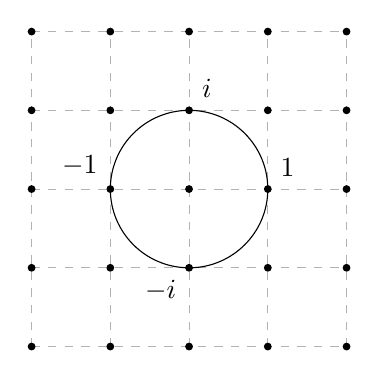
\begin{tikzpicture}[x=1cm, y=1cm]

      \foreach \i in {-2,...,2}
      \draw[black!30,dashed] (\i,-2) -- (\i,2);

      \foreach \j in {-2,...,2}
      \draw[black!30,dashed] (-2,\j) -- (2,\j);

      \draw (-2,0) node[circle,fill,inner sep=1pt] {};
      \draw (-1,0) node[circle,fill,inner sep=1pt, label=above left:{$-1$}] {};
      \draw (0,0) node[circle,fill,inner sep=1pt] {};
      \draw (1,0) node[circle,fill,inner sep=1pt, label=above right:{$1$}] {};
      \draw (2,0) node[circle,fill,inner sep=1pt] {};

      \draw (-2,1) node[circle,fill,inner sep=1pt] {};
      \draw (-1,1) node[circle,fill,inner sep=1pt] {};
      \draw (0,1) node[circle,fill,inner sep=1pt, label=above right:{$i$}] {};
      \draw (1,1) node[circle,fill,inner sep=1pt] {};
      \draw (2,1) node[circle,fill,inner sep=1pt] {};

      \draw (-2,-1) node[circle,fill,inner sep=1pt] {};
      \draw (-1,-1) node[circle,fill,inner sep=1pt] {};
      \draw (0,-1) node[circle,fill,inner sep=1pt, label=below left:{$-i$}] {};
      \draw (1,-1) node[circle,fill,inner sep=1pt] {};
      \draw (2,-1) node[circle,fill,inner sep=1pt] {};

      \draw (-2,2) node[circle,fill,inner sep=1pt] {};
      \draw (-1,2) node[circle,fill,inner sep=1pt] {};
      \draw (0,2) node[circle,fill,inner sep=1pt] {};
      \draw (1,2) node[circle,fill,inner sep=1pt] {};
      \draw (2,2) node[circle,fill,inner sep=1pt] {};

      \draw (-2,-2) node[circle,fill,inner sep=1pt] {};
      \draw (-1,-2) node[circle,fill,inner sep=1pt] {};
      \draw (0,-2) node[circle,fill,inner sep=1pt] {};
      \draw (1,-2) node[circle,fill,inner sep=1pt] {};
      \draw (2,-2) node[circle,fill,inner sep=1pt] {};

      \draw (0,0) circle (1);
    \end{tikzpicture}
  \end{center}

  \caption{Unidades en los enteros de Gauss $\ZZ [i]$}
\end{figure}

\begin{ejemplo}
  Calcular los elementos invertibles en un anillo no es tan fácil como uno puede
  pensar. Por ejemplo, tenemos
  $$\frac{1}{1 + \sqrt{2}} = \frac{1 - \sqrt{2}}{(1 + \sqrt{2})\,(1 - \sqrt{2})} = \frac{1-\sqrt{2}}{1 - 2} = -1 + \sqrt{2},$$
  así que $1 + \sqrt{2}$ es invertible en el anillo $\ZZ [\sqrt{2}]$. Luego,
  todas las potencias de $1 + \sqrt{2}$ son también invertibles: para cualquier
  $n = 2,3,4,\ldots$
  $$((1+\sqrt{2})^n)^{-1} =  ((1+\sqrt{2})^{-1})^n = (-1 + \sqrt{2})^n \in \ZZ [\sqrt{2}].$$
  Los números $(1+\sqrt{2})^n$ son diferentes:
  $$1+\sqrt{2} < (1+\sqrt{2})^2 < (1+\sqrt{2})^3 < (1+\sqrt{2})^4 < \cdots$$
  Entonces, en el anillo $\ZZ [\sqrt{2}]$ hay un número infinito de unidades.
\end{ejemplo}

\begin{ejemplo}
  \label{ejemplo:grupo-de-unidades-de-ZnZ}
  Un número $a\in \ZZ$ es invertible módulo $n = 1,2,3,\ldots$ si y solamente si
  $\mcd (a,n) = 1$:
  $$(\ZZ/n\ZZ)^\times = \{ [a]_n \mid \mcd (a,n) = 1 \}.$$
  En particular,
  \begin{align*}
    (\ZZ/2\ZZ)^\times & = \{ [1]_1 \},\\
    (\ZZ/3\ZZ)^\times & = \{ [1]_3, [2]_3 \},\\
    (\ZZ/4\ZZ)^\times & = \{ [1]_4, [3]_4 \},\\
    (\ZZ/5\ZZ)^\times & = \{ [1]_5, [2]_5, [3]_5, [4]_5 \},\\
    (\ZZ/6\ZZ)^\times & = \{ [1]_6, [5]_6 \},\\
    (\ZZ/7\ZZ)^\times & = \{ [1]_7, [2]_7, [3]_7, [4]_7, [5]_7, [6]_7 \},\\
    (\ZZ/8\ZZ)^\times & = \{ [1]_8, [3]_8, [5]_8, [7]_8 \},\\
    (\ZZ/9\ZZ)^\times & = \{ [1]_9, [2]_9, [4]_9, [5]_9, [7]_9, [8]_9 \},\\
    (\ZZ/10\ZZ)^\times & = \{ [1]_{10}, [3]_{10}, [7]_{10}, [9]_{10} \},\\
                      & \cdots
  \end{align*}

  En efecto, asumamos que $\mcd (a,n) = 1$. Entonces, la
  \term{identidad de Bézout} nos da
  $$ab + nc = 1$$
  para algunos $b,c \in \ZZ$. Luego, $ab \equiv 1 \pmod{n}$, así que
  $[a]_n^{-1} = [b]_n$.

  Viceversa, asumamos que para $[a]_n$ existe $[b]_n$ tal que
  $[a]_n\cdot [b]_n = 1$. Luego, $ab \equiv 1 \pmod{n}$, lo que significa que
  $$ab + nc = 1.$$
  para algún $c \in \ZZ$. Pero esta identidad implica que
  $\mcd (a,n) = 1$. (Recordemos que $\mcd (a,n)$ es el mínimo número positivo de
  la forma $ax + ny$ para $x,y\in\ZZ$.)
\end{ejemplo}

La función
$$\phi (n) \dfn |(\ZZ/n\ZZ)^\times| = \# \{ 0 \le a \le n-1 \mid \mcd (a,n) = 1 \}$$
se llama la
\term{función $\phi$ de Euler}. He aquí
algunos de sus valores:

\begin{center}\small
  \begin{tabular}{rx{0.35cm}x{0.35cm}x{0.35cm}x{0.35cm}x{0.35cm}x{0.35cm}x{0.35cm}x{0.35cm}x{0.35cm}x{0.35cm}x{0.35cm}x{0.35cm}x{0.35cm}x{0.35cm}x{0.35cm}x{0.35cm}}
    \hline
    $n\colon$ & $1$ & $2$ & $3$ & $4$ & $5$ & $6$ & $7$ & $8$ & $9$ & $10$ & $11$ & $12$ & $13$ & $14$ & $15$  \tabularnewline
    $\phi (n)\colon$ & $1$ & $1$ & $2$ & $2$ & $4$ & $2$ & $6$ & $4$ & $6$ & $4$ & $10$ & $4$ & $12$ & $6$ & $8$ \tabularnewline
    \hline
    $n\colon$ & $16$ & $17$ & $18$ & $19$ & $20$ & $21$ & $22$ & $23$ & $24$ & $25$ & $26$ & $27$ & $28$ & $29$ & $30$ \tabularnewline
    $\phi (n)\colon$ & $8$ & $16$ & $6$ & $18$ & $8$ & $12$ & $10$ & $22$ & $8$ & $20$ & $12$ & $18$ & $12$ & $28$ & $8$ \tabularnewline
    \hline
  \end{tabular}
\end{center}

\begin{proposicion}
  Si $p = 2,3,5,7,11,\ldots$ es primo y $k = 1,2,3,4,\ldots$, entonces
  $$\phi (p^k) = p^k\,\left(1 - \frac{1}{p}\right).$$

  \begin{proof}
    Consideramos los números
    $$a = 0, 1, 2, \ldots, p^k-2, p^k-1.$$
    En esta lista hay $p^k$ elementos. Luego, $\mcd (a,p^k) = 1$ si y solamente
    si $p\nmid a$. Los números en la esta tales que $p\mid a$ son los múltiplos
    de $p$: $0, p, 2p, 3p, \ldots$---cada $p$-ésimo número, en total $p^k / p$
    de ellos. Entonces,
    \[ \phi (p^k) = p^k - \frac{p^k}{p} = p^k\,\left(1 - \frac{1}{p}\right). \qedhere \]
  \end{proof}
\end{proposicion}

% % % % % % % % % % % % % % % % % % % % % % % % % % % % % %

\section{Cuerpos}

\begin{definicion}
  Un \term{cuerpo} $k$ es un anillo conmutativo tal que

  \begin{enumerate}
  \item[1)] $k \ne 0$,

  \item[2)] todo elemento no nulo de $k$ es invertible.
  \end{enumerate}
\end{definicion}

\begin{ejemplo}
  Los anillos $\QQ$, $\RR$, $\CC$ son cuerpos.
\end{ejemplo}

\begin{ejemplo}
  El cuerpo más pequeño posible consiste en dos elementos $0$ y $1$ con las
  siguientes operaciones:

  \begin{center}
    \begin{tabular}{f{0.5cm}|f{0.5cm}f{0.5cm}}
      $+$ & $0$ & $1$ \tabularnewline
      \hline
      $0$ & $0$ & $1$ \tabularnewline
      $1$ & $0$ & $0$
    \end{tabular}
    \quad\quad
    \begin{tabular}{f{0.5cm}|f{0.5cm}f{0.5cm}}
      $\cdot$ & $0$ & $1$ \tabularnewline
      \hline
      $0$ & $0$ & $0$ \tabularnewline
      $1$ & $0$ & $1$
    \end{tabular}
  \end{center}
\end{ejemplo}

\begin{ejemplo}
  Para $n\ne 1$ un entero libre de cuadrados, consideremos el anillo
  $$\QQ (\sqrt{n}) \dfn \{ a + b\sqrt{n} \mid a,b\in \QQ \}.$$
  Este es un cuerpo: para $a + b\sqrt{n} \ne 0$ calculamos
  \[ (a + b\sqrt{n})^{-1} =
    \frac{a - b\sqrt{n}}{(a + b\sqrt{n})\,(a - b\sqrt{n})} =
    \frac{a}{a^2-nb^2} - \frac{b}{a^2-nb^2}\,\sqrt{n} \in \QQ (\sqrt{n}). \]
  Aquí es importante que $a^2 - nb^2 \ne 0$ si $(a,b) \ne (0,0)$. En efecto,
  si $n < 0$, tenemos una suma de $a^2$ y un múltiplo positivo de $b^2$ que
  puede ser nula solo cuando $a = b = 0$. Si $n > 0$, entonces $a^2 - nb^2 = 0$
  implica que $n = \left(\frac{a}{b}\right)^2$ que no es el caso porque $n$ es
  libre de cuadrados.
\end{ejemplo}

La existencia de elementos inversos en un cuerpo garantiza que es un dominio.

\begin{observacion}
  Todo cuerpo es un dominio.

  \begin{proof}
    Supongamos que $xy = 0$, donde $x \ne 0$. Si estamos en un cuerpo, para $x$
    existe su inverso $x^{-1}$, y multiplicando la identidad $xy = 0$ por
    $x^{-1}$, se obtiene
    $$x^{-1} (xy) = x^{-1}\cdot 0,$$
    donde la parte izquierda es igual a $(x^{-1} x)\,y = 1\cdot y = y$,
    y la parte derecha es igual a $0$.
  \end{proof}
\end{observacion}

\begin{proposicion}
  $\ZZ/n\ZZ$ es un cuerpo si y solamente si $n = p$ es primo.

  \begin{proof}
    Si $n = p$ es primo, entonces $\mcd (a,p) = 1$ para todo $a = 1,\ldots,p-1$
    y todos los restos no nulos $[1]_p, [2]_p, \ldots, [p-1]_p$ son
    invertibles. Si $n$ es compuesto, ya hemos notado que $\ZZ/n\ZZ$ no es un
    dominio, y en particular no es un cuerpo.
  \end{proof}
\end{proposicion}

\begin{notacion}
  Para un número primo $p$ el cuerpo $\ZZ/p\ZZ$ se denota por $\FF_p$.
\end{notacion}

\begin{ejemplo}
  Sea $\FF_4$ el espacio vectorial de dimensión $2$ sobre el cuerpo $\FF_2$,
  generado por los elementos $1$ y $\alpha$. Este espacio tiene $4$ elementos:
  $$\FF_4 = \{ 0, 1, \alpha, \alpha+1 \}.$$
  La adición de vectores nos da
  \begin{center}
    \begin{tabular}{c|f{1cm}f{1cm}f{1cm}f{1cm}}
      $+$ & $0$ & $1$ & $\alpha$ & $\alpha+1$ \tabularnewline
      \hline
      $0$ & $0$ & $1$ & $\alpha$ & $\alpha+1$ \tabularnewline
      $1$ & $1$ & $0$ & $\alpha+1$ & $\alpha$ \tabularnewline
      $\alpha$ & $\alpha$ & $\alpha+1$ & $0$ & $1$ \tabularnewline
      $\alpha+1$ & $\alpha+1$ & $\alpha$ & $1$ & $0$
    \end{tabular}
  \end{center}
  Definamos la multiplicación mediante $0\cdot x = x\cdot 0 = 0$,
  $1\cdot x = x\cdot 1 = x$ para todo $x$ y la identidad
  $$\alpha^2 + \alpha + 1 = 0.$$
  Luego,
  $$\alpha\,(\alpha+1) = \alpha^2 + \alpha = 1$$
  y
  $$(\alpha+1)^2 = \alpha^2 + 1^2 = \alpha.$$

  \begin{center}
    \begin{tabular}{c|f{1cm}f{1cm}f{1cm}f{1cm}}
      $\cdot$ & $0$ & $1$ & $\alpha$ & $\alpha+1$ \tabularnewline
      \hline
      $0$ & $0$ & $0$ & $0$ & $0$ \tabularnewline
      $1$ & $0$ & $1$ & $\alpha$ & $\alpha+1$ \tabularnewline
      $\alpha$ & $0$ & $\alpha$ & $\alpha+1$ & $1$ \tabularnewline
      $\alpha+1$ & $0$ & $\alpha+1$ & $1$ & $\alpha$
    \end{tabular}
  \end{center}
  Se puede verificar que lo que tenemos es un cuerpo de cuatro elementos.
\end{ejemplo}

\begin{digresion}
  En general, todo cuerpo finito necesariamente tiene orden $q = p^k$ donde
  $p = 2, 3, 5, 7, 11, \ldots$ es primo y $k = 1, 2, 3, 4, \ldots$ Estos cuerpos
  se denotan por $\FF_{p^k}$. Cuando $k = 1$, es la misma cosa que $\ZZ/p\ZZ$,
  pero para $k > 1$, como hemos notado, $\ZZ/p^k\ZZ$ no es un cuerpo, así que
  $\FF_{p^k}$ tiene construcción diferente. Vamos a estudiarlo en la
  continuación de este curso.
\end{digresion}

\begin{definicion}
  Si $L$ es un cuerpo y $K \subseteq L$ es su subanillo que es también un
  cuerpo. En este caso se dice que $K$ es un \term{subcuerpo} de $L$. También se
  dice que $K \subseteq L$ es una \term{extensión de cuerpos}.
\end{definicion}

\begin{observacionejerc}
  Si $K \subseteq L$ es una extensión de cuerpos, entonces $L$ es un espacio
  vectorial sobre $K$ respecto a la suma en $L$ y la multiplicación de los
  elementos de $L$ por elementos de $K$.
\end{observacionejerc}

\begin{ejemplo}
  Hemos visto las siguientes extensiones de cuerpos:
  $$\QQ \subset \RR \subset \CC, \quad \QQ \subset \QQ (\sqrt{n}) \subset \CC.$$
  El cuerpo $\FF_4 = \{ 0, 1, \alpha, \alpha+1 \}$ que hemos construido arriba
  contiene un subcuerpo $\FF_2 = \{ 0, 1 \}$.
\end{ejemplo}

% % % % % % % % % % % % % % % % % % % % % % % % % % % % % %

\section{Cuerpos de fracciones}

\epigraph{Un hombre es como una fracción cuyo numerador es lo que es y cuyo
  denominador es lo que él piensa de sí mismo.}{León Tolstoi}

La construcción de los números racionales $\QQ$ a partir de los números enteros
$\ZZ$ puede ser generalizada a cualquier dominio.

\begin{construccion}
  Sea $A$ un dominio. Consideremos la siguiente relación sobre
  $A\times A\setminus \{ 0 \}$:
  $$(a,b) \sim (a',b') \iff ab' = a'b.$$
  Esta relación es visiblemente reflexiva y simétrica. Para ver que es
  transitiva, notamos que si
  $$(a,b) \sim (a,b), \quad (a',b') \sim (a'',b''),$$
  entonces
  $$ab' = a'b, \quad a'b'' = a''b'.$$
  Luego, usando que $A$ es conmutativo (!)
  $$b' \, (ab'') = (ab')\,b'' = (a'b)\,b'' = b\,(a'b'') = b\,(a'' b') = b'\,(a''b).$$
  Dado que $A$ es un dominio (!), podemos cancelar $b'$ y concluir que
  $ab'' = a''b$; es decir, que $(a,b) \sim (a'',b'')$.

  Denotemos la clase de equivalencia de $(a,b)$ por la fracción
  $$\frac{a}{b} \dfn [(a,b)]$$
  y pongamos
  $$\Frac A \dfn (A\times A\setminus \{ 0 \})/\!\sim = \Bigl\{ \frac{a}{b} \Bigm| a,b\in A, ~ b\ne 0 \Bigr\}.$$
  Definamos la suma y producto de fracciones mediante
  \[ \frac{a}{b} + \frac{c}{d} \dfn \frac{ad + cb}{bd}, \quad
    \frac{a}{b}\cdot\frac{c}{d} \dfn \frac{ac}{bd}. \]
\end{construccion}

\begin{observacionejerc}
  Las operaciones de arriba están bien definidas y definen una estructura de
  anillo conmutativo sobre $\Frac A$. El cero es la fracción $\frac{0}{1}$ y
  la identidad es la fracción $\frac{1}{1}$.
\end{observacionejerc}

Notamos que una fracción es nula precisamente cuando su numerador es nulo:
$$\frac{a}{b} = \frac{0}{1} \iff a = 0.$$
Ahora toda fracción $\frac{a}{b} \ne \frac{0}{1}$ admite inversa:
$$\left(\frac{a}{b}\right)^{-1} = \frac{b}{a}.$$
Esto significa que $\Frac A$ es un cuerpo.

Notamos que tenemos la aplicación inyectiva $a \mapsto \frac{a}{1}$:
$$\frac{a}{1} = \frac{a'}{1} \iff a = a'.$$
De esta manera las fracciones con $1$ en el numerador pueden ser identificadas
con $A$.

\begin{definicion}
  Para un dominio $A$, el cuerpo $\Frac A$ que acabamos de construir se llama el
  \term{cuerpo de fracciones} de $A$.
\end{definicion}

\begin{ejemplo}
  El cuerpo de fracciones de $\ZZ$ es precisamente $\QQ$.
\end{ejemplo}

\begin{ejemplo}
  Sea $k$ un cuerpo. Entonces, los polinomios con coeficientes en $k$ forman un
  dominio $k [X]$. El cuerpo de fracciones correspondiente viene dado por
  $$k (X) \dfn \Frac k[X] = \Bigl\{ \frac{f}{g} \Bigm| f,g \in A [X], ~ g\ne 0 \Bigr\}.$$
  Por ejemplo, tenemos en $k (X)$
  \[ \frac{X^n-1}{1} \cdot \frac{1}{X-1} = \frac{1 + X + X^2 + \cdots + X^{n-1}}{1}. \qedhere \]
\end{ejemplo}

\begin{ejemplo}
  Si $k$ es un cuerpo, no es muy interesante tomar el cuerpo de fracciones
  $\Frac k$. En efecto, tendremos para toda fracción
  $$\frac{a}{b} = \frac{ab^{-1}}{bb^{-1}} = \frac{ab^{-1}}{1},$$
  así que en el denominador siempre se puede poner $1$. De esta manera $\Frac k$
  se identifica con el mismo $k$, pero las palabras ``se identifica'' tendrán un
  sentido preciso un poco más adelante.
\end{ejemplo}

Vamos a volver a los cuerpos de fracciones más adelante, después de introducir
la noción de homomorfismo e isomorfismo de anillos.

% % % % % % % % % % % % % % % % % % % % % % % % % % % % % %

\section{¿Para qué sirven los anillos? ($\clubsuit$)}

Los anillos conmutativos tienen mucha importancia en las matemáticas
modernas. En muchas situaciones hay una correspondencia
$$\text{Objetos geométricos (``espacios'')} \longleftrightarrow \text{Objetos algebraicos hechos de anillos conmutativos}.$$
A veces para solucionar problemas geométricos, se puede pasar a los objetos
algebraicos correspondientes. Por otro lado, hay muchos objetos algebraicos que
surgen naturalmente en la teoría de números; un ejemplo básico son los anillos
como $\ZZ$, $\ZZ [i]$, $\ZZ [\sqrt{n}]$ que hemos visto arriba. A tales objetos
se pueden asociar ciertos ``espacios'' y aplicar la intuición geométrica para
resolver problemas aritméticos. Es uno de los temas principales de las
matemáticas a partir de los años 50--60 del siglo pasado. Preguntar a un
matemático moderno si él prefiere trabajar con objetos algebraicos o usar la
intuición geométrica es como preguntarse si uno prefiere quedarse ciego o sordo.

\vspace{1em}

Los cuerpos son un caso muy especial de anillos, y de hecho, bajo la
correspondencia geométrica-algebraica que mencioné, a un cuerpo corresponde un
espacio que consiste solo de un punto. Los anillos $\ZZ$, $\ZZ [i]$,
$\ZZ [\sqrt{n}]$ son también bastante sencillos: si los cuerpos tienen dimensión
$0$, estos tienen dimensión~$1$. Hay anillos de dimensiones superiores, por
ejemplo si consideramos el anillo de polinomios $A [X]$, la dimensión sube por
$1$:
$$\dim A [X] = \dim A + 1.$$
En particular, la dimensión de $k [X]$ para un cuerpo $k$ es igual a
$1$. También hay anillos de dimensión infinita, pero no los vamos a encontrar en
este curso.
